\documentclass[12pt,a4paper]{article}

\usepackage[a4paper,margin=1in]{geometry}
\usepackage{graphicx}
\usepackage{booktabs}
\usepackage{amsmath,amssymb}
\usepackage{float}
\usepackage{hyperref}
\usepackage{xcolor}
\usepackage{listings}
\usepackage{enumitem}
\usepackage{fancyhdr}
\usepackage{longtable}

\usepackage{xurl}
\setlength{\emergencystretch}{3em}
\hypersetup{colorlinks=true,linkcolor=blue,urlcolor=blue}

\pagestyle{fancy}
\fancyhf{}
\lhead{ICS1512}
\rhead{Machine Learning Algorithms Laboratory}
\cfoot{\thepage}

\lstset{
language=Python,
basicstyle=\ttfamily\small,
numbers=left,
frame=single,
breaklines=true,
showstringspaces=false
}

\begin{document}

\begin{tabular}{|p{4cm}|p{11cm}|}
\hline
Experiment No. & 9 \\ \hline
Experiment Title & Perceptron vs Multilayer Perceptron (A/B Experiment) with Hyperparameter
Tuning\footnotemark\\ \hline
Student Name & Simiyon Vinscent Samuel L \\ \hline
Register Number & 3122247001062 \\ \hline
Faculty & Dr. Poreddy Ajay Kumar Reddy \\ \hline
Submission Date & August 2, 2026 \\ \hline
\end{tabular}
\footnotetext{\textbf{GitHub Repository: }\url{https://github.com/blackscythe123/Machine-Learning-course}}

\section{Objective}
\begin{itemize}[nosep]
\item To implement a single-layer Perceptron Learning Algorithm (PLA) from scratch with a step
activation and the rule $w_{t+1} = w_t + \eta\,(y - \hat{y})\,x$ (Model A).
\item To implement a Multilayer Perceptron (MLP) with hidden layers and nonlinear activations,
trained by backpropagation (Model B).
\item To choose the MLP's activation function, cost function, optimizer, learning rate, batch
size, depth and width through systematic tuning on a held-out validation set.
\item To compare PLA and the tuned MLP on the test set with accuracy, precision, recall, F1,
confusion matrices, ROC curves and training-error curves, and to study overfitting and how to
reduce it.
\end{itemize}

\section{Problem Statement}
Recognise a handwritten character from a picture of it. Each image shows one of 62 characters
(the digits 0 to 9, the uppercase letters A to Z and the lowercase letters a to z), so this is a
62-class classification problem with only 55 examples per class. The two models are the same in
spirit, a weighted sum of the pixels followed by a decision, but the perceptron uses one layer of
weights and a hard threshold, whereas the MLP stacks layers with smooth nonlinearities. The
experiment measures how much that difference is worth, and how much of the MLP's result depends
on tuning choices such as the optimizer and the cost function.

\section{Dataset Description}
\begin{longtable}{|p{6cm}|p{8cm}|}
\hline
Dataset Name & English Handwritten Characters \\ \hline
Dataset Source & Kaggle
(\url{https://www.kaggle.com/datasets/dhruvildave/english-handwritten-characters-dataset}), the
link given in the assignment \\ \hline
Number of Samples & 3410 images \\ \hline
Image Format & PNG, $1200 \times 900$ pixels, black strokes on a white background (each pixel
is either black or white in the files) \\ \hline
Number of Classes & 62 (10 digits, 26 uppercase letters, 26 lowercase letters), exactly 55
images per class \\ \hline
Character Types & Digits 550 (16.1\%), uppercase 1430 (41.9\%), lowercase 1430 (41.9\%) \\ \hline
Missing Values & 0 (every listed file exists and every image has a label) \\ \hline
Train / Validation / Test Split & 70\% / 15\% / 15\%, stratified on the class label
(\texttt{random\_state=42}): 2386 training, 512 validation and 512 test images (38 or 39 per class in training, 8 or 9 per class in validation and test) \\ \hline
\end{longtable}

\section{Exploratory Data Analysis}
\begin{figure}[H]
\centering

\includegraphics[width=\linewidth]{figures/00_eda_summary.png}
\caption{Consolidated exploratory data analysis (12 subplots, single page): (1) images per character type;
(2) a raw image with the bounding box of its ink; (3) the mean image of each of the 62 classes; (4, 5, 6) the
distributions of ink coverage, ink-box height and ink-box aspect ratio by character type; (7) boxplot of ink
coverage; (8) pixel variance map of the $32 \times 32$ inputs; (9) correlation between the 62 class-mean images
(white lines separate digits, uppercase and lowercase); (10) PCA projection coloured by character type; (11)
cumulative explained variance of the first 200 principal components; (12) total ink in each $32 \times 32$ image.
Exported at 600 DPI as \texttt{figures/00\_eda\_summary.eps} and reproduced here as PNG.}
\end{figure}

\textbf{Inference:} The dataset is balanced by class (55 images each) but not by type, since letters
outnumber digits (there are 26 letters of each case but only 10 digits). The raw drawings occupy a small part of the
canvas: the median ink share is 5.6\% for digits, 6.4\% for uppercase letters and 4.8\% for lowercase letters,
and lowercase characters are shorter (median ink-box height 382 px against 452 px for digits and 478 px for
uppercase letters) with a longer tail of wide boxes. The class-mean images are recognisable, blurred versions of
the characters, so each class has a consistent shape despite the many writing styles. The pixel variance is
concentrated in the central part of the square and close to zero at the border, which is where the crop and
margin put the ink. The class-mean correlations show that some classes are close to duplicates of others: the
class-mean images of an uppercase letter and its lowercase twin have a mean correlation of 0.73, against 0.48
for an uppercase and a lowercase letter that differ, and the pairs V and v (0.95), W and w (0.93), P and p
(0.90) and S and s (0.90) are the most similar. The digit 0 and the letter O (0.91) and the letter I and l
(0.93) are similar in the same way. Scatter of the first two principal components shows no separation of
the three character types, and 32 components are needed for 80\% of the variance, 65 for 90\% and 132 for
95\% (the 200 components shown retain 97.1\%), so the data is not low-dimensional.


\section{Data Preprocessing}
\begin{itemize}
\item \textbf{Missing values and labels:} None missing. The labels are the characters
themselves (a string per class) and were mapped to the integers 0 to 61 in sorted order
(digits, then uppercase, then lowercase).
\item \textbf{Cropping:} Each drawing sits somewhere on a large $1200 \times 900$ canvas and
fills only about 5\% of it. The bounding box of the black pixels was cut out, so the character
itself, not the blank canvas, is what the models see.
\item \textbf{Padding to a square:} The cropped box was centred on a square black canvas whose
side is 1.2 times the longer side of the box (a 10\% margin on each side), so the aspect ratio
of the character is kept instead of being stretched.
\item \textbf{Inversion and resizing:} Ink was made the high value (white strokes on black
during processing, drawn as dark ink in the figures) and the square was resized to
$32 \times 32$ with Lanczos resampling, giving 1024 features per image. The strokes in the
originals are thick, so the characters stay readable at this size (Figure~\ref{fig:prep}).
\item \textbf{Flattening and normalising:} Each image was flattened to a vector of 1024 values
and divided by 255 so that every pixel lies in $[0, 1]$.
\item \textbf{Standardisation (PLA only, tested):} A \texttt{StandardScaler} fitted on the
training split only was tried as an alternative input for the perceptron. The MLP uses the
plain $[0, 1]$ pixels.
\item \textbf{Splitting:} 70/15/15 stratified train, validation and test split. All tuning
decisions use the validation split; the test split was used only for the final comparison.
\end{itemize}

\begin{figure}[H]
\centering
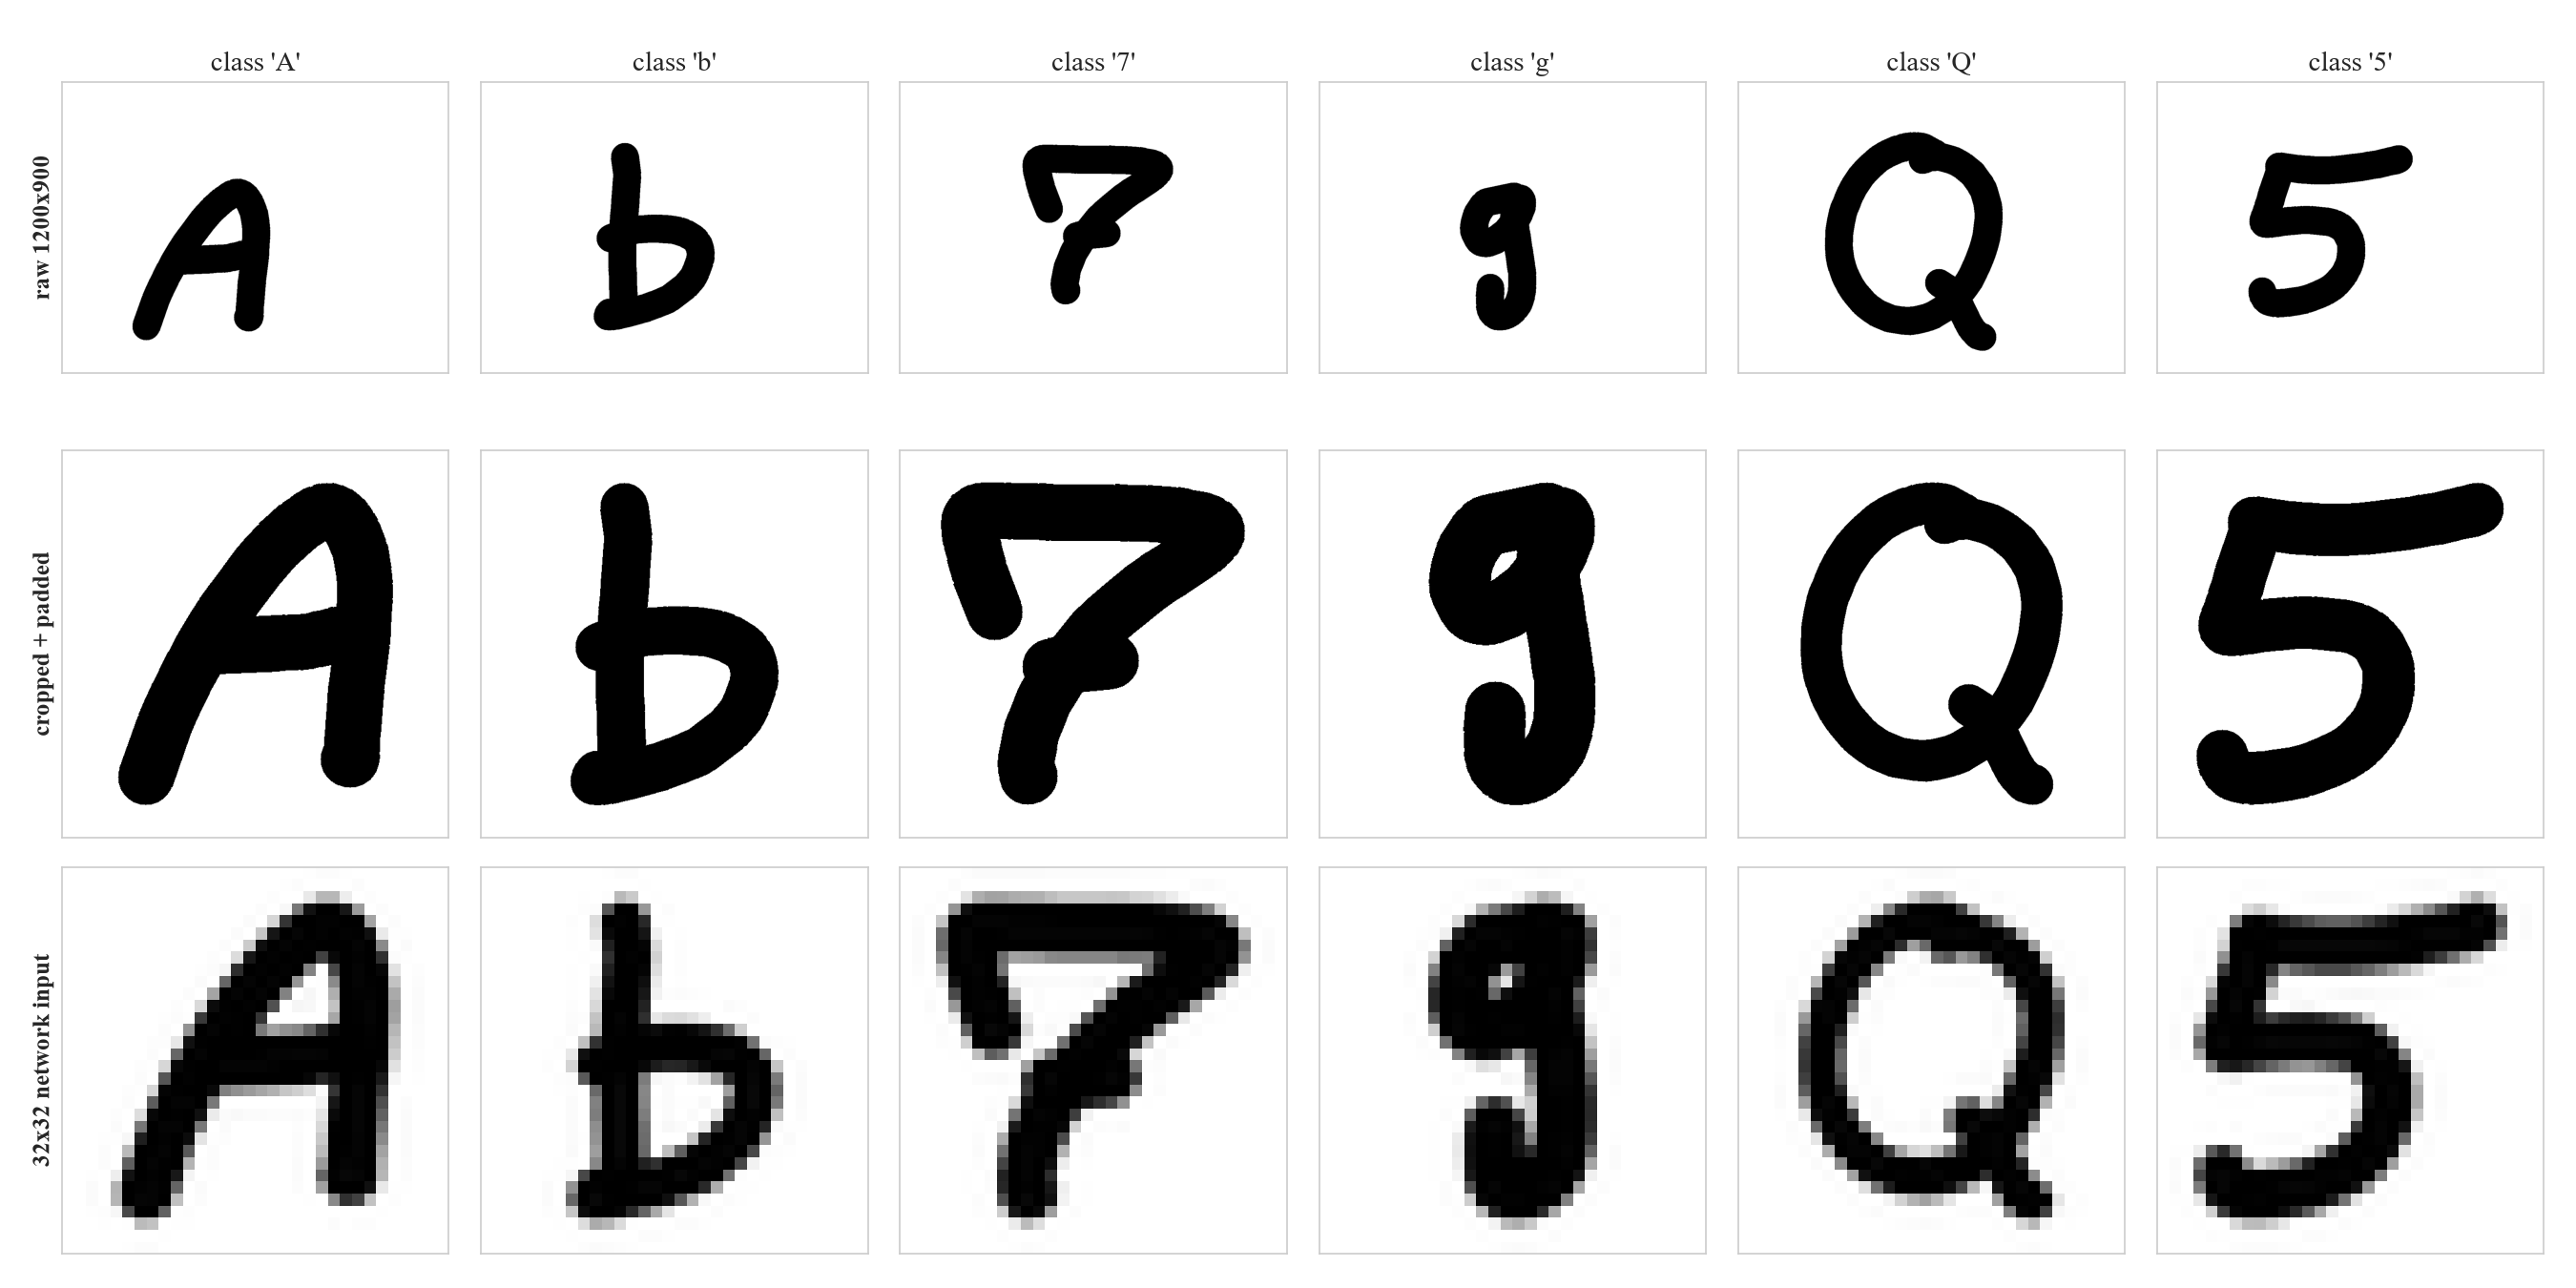
\includegraphics[width=\linewidth]{figures/01_preprocessing_steps.png}
\caption{Preprocessing of six sample images: the raw $1200 \times 900$ drawing (top), after
cropping to the ink and padding to a square (middle), and the $32 \times 32$ network input
(bottom).}
\label{fig:prep}
\end{figure}
\textbf{Inference:} The crop makes every character fill its square, which removes the large and
varying blank margins of the raw canvas. The strokes are thick enough that all six characters remain
easy to read at $32 \times 32$. The crop also discards the absolute size of a character, an
information loss that matters for letters such as v and V (see the Discussion).

\section{Machine Learning Algorithm}

\subsection*{Model A: Perceptron Learning Algorithm}
A perceptron computes $\hat{y} = \text{step}(w^{\top}x + b)$, where $\text{step}(z)$ is 1 if
$z > 0$ and 0 otherwise. When it makes a mistake on an example it moves the weights toward the
correct answer with the update
\[
w_{t+1} = w_t + \eta\,(y - \hat{y})\,x .
\]
For 62 classes a one-vs-rest scheme was used: there is one perceptron per character (62 weight
vectors and 62 biases, $1025 \times 62 = 63{,}550$ parameters in total), trained on the target
``is this image character $k$?''. At prediction time the class with the largest score
$w_k^{\top}x + b_k$ is chosen. The whole algorithm, the shuffling, the step activation and the
update rule, is written in \texttt{numpy} inside a \texttt{Perceptron} class; no library
implementation is used. Weights start at zero, and each epoch visits the training images once in
a random order.

A perceptron only converges when the classes are linearly separable. If they are not, it keeps
making mistakes and its weights keep changing, so the epoch at which training is stopped matters
and was chosen on the validation set.

\subsection*{Model B: Multilayer Perceptron}
The MLP maps the 1024 inputs through one or more fully connected hidden layers, each followed by a
nonlinear activation (ReLU, tanh or sigmoid), to 62 output scores. Training uses backpropagation
to compute the gradient of a cost function and an optimizer to take the step. It was implemented
in PyTorch and trained on the GPU. The options studied were:
\begin{itemize}
\item \textbf{Activation:} ReLU, tanh, sigmoid.
\item \textbf{Cost function:} cross-entropy on the softmax output, and mean squared error between
the softmax output and the one-hot label.
\item \textbf{Optimizer:} full-batch gradient descent (GD), mini-batch stochastic gradient descent
(SGD), SGD with momentum 0.9, and Adam.
\item \textbf{Learning rate:} 0.001, 0.01, 0.1.
\item \textbf{Batch size:} 32, 128, 512 (full batch for GD).
\item \textbf{Architecture:} 0 to 5 hidden layers, and 64 to 1024 neurons per layer.
\item \textbf{Regularisation:} dropout, L2 weight decay, early stopping and random-affine data
augmentation.
\end{itemize}

\subsection*{Evaluation Metrics}
\begin{itemize}
\item \textbf{Accuracy} is the fraction of test images classified correctly.
\item \textbf{Precision, recall and F1} are computed per class and then averaged with equal
weight (macro average), so each of the 62 characters counts the same.
\item \textbf{Confusion matrix:} rows are true characters, columns are predicted characters.
\item \textbf{ROC curves:} one-vs-rest curves from the class scores; the \emph{micro} average
pools all image-class decisions, and the \emph{macro} average averages the 62 per-class curves
with equal weight. For the MLP the softmax probabilities are the scores; for the PLA the raw
scores $w_k^{\top}x + b_k$ are used.
\item \textbf{Training error against epochs:} the misclassification rate on the training split
after every epoch.
\end{itemize}

\section{Experimental Setup}
\begin{tabular}{lp{10.5cm}}
\toprule
Python Version & 3.13.14 \\
NumPy Version & 2.5.1 \\
Scikit-Learn Version & 1.9.0 \\
PyTorch Version & 2.11.0 (CUDA 12.8 build) \\
IDE & Jupyter Notebook \\
Operating System & Windows 11 \\
Hardware & Intel Core Ultra 9, NVIDIA GeForce RTX 5060 Laptop GPU (8 GB), used for the MLP \\
PLA Hardware & CPU (\texttt{numpy}) \\
\bottomrule
\end{tabular}

\section{Hyperparameter Selection}
Every tuning decision was made on the 512-image validation split. The 512-image test split was
used once, at the end, for the PLA against MLP comparison. The search spaces are below; the
first MLP stage is a full grid, and later stages change one design choice at a time around the
grid winner.

\begin{longtable}{p{3.0cm}p{3.2cm}p{8.0cm}}
\toprule
Model & Setting & Values tried \\
\midrule
PLA & Input scaling & pixels in $[0,1]$; standardized pixels (\texttt{StandardScaler}, fitted on the
training split) \\
PLA & Learning rate $\eta$ & 0.01, 0.1, 1.0 \\
PLA & Epochs & trained for 100 epochs; the epoch count with the lowest validation error (seed 42)
was then used for every final perceptron \\
MLP grid & Activation & ReLU, tanh, sigmoid \\
MLP grid & Cost function & cross-entropy (CE), mean squared error (MSE) \\
MLP grid & Optimizer & GD (full batch), SGD, SGD with momentum 0.9, Adam \\
MLP grid & Learning rate & 0.001, 0.01, 0.1 \\
MLP grid & Batch size & 32, 128, 512 (all 2386 training images for GD) \\
MLP grid & Architecture & one hidden layer of 256 neurons, 100 epochs, seed 42 \\
MLP follow-up & Depth & 0 to 5 hidden layers of 256 neurons; repeated for each activation with
Adam, learning rate 0.001, batch 128, CE \\
MLP follow-up & Width & 64, 128, 256, 512, 1024 neurons \\
MLP follow-up & Regularisation & dropout 0, 0.2, 0.4 crossed with weight decay 0, $10^{-4}$,
$10^{-3}$; early stopping (patience 10); random-affine data augmentation \\
\bottomrule
\end{longtable}

The grid has $3 \times 2 = 6$ activation and cost pairs, and each pair has $3$ GD runs (one batch
size) plus $3 \times 3 \times 3 = 27$ runs for the other three optimizers, so $6 \times 30 = 180$
runs. Each grid run is scored by the validation accuracy of the model after its last epoch. The
six best runs were then repeated with four seeds (42, 1, 2, 3), because a single validation split
of 512 images cannot separate configurations that differ by less than about one point. Later
stages report the mean over the same four seeds.

\section{Results}

\subsection*{Model A: PLA}
{\small\setlength{\tabcolsep}{4pt}
\begin{longtable}{p{3.3cm}p{2.3cm}p{2.2cm}p{2.2cm}p{2.0cm}p{1.6cm}}
\toprule
Input & $\eta$ & Train acc.\ (epoch 100) & Val.\ acc.\ (epoch 100) & Best val.\ acc. & Best epoch \\*
\midrule
pixels in $[0,1]$ & 0.01, 0.1, 1.0 & 0.9975 & 0.6855 & 0.6973 & 77 \\
standardized pixels & 0.01, 0.1, 1.0 & 0.9916 & 0.5059 & 0.5137 & 47 \\
\bottomrule
\end{longtable}
}

\textbf{Inference:} The perceptron fits the training images almost perfectly (training accuracy
99.7\%) yet reaches only
69.7\% on the validation split, so it is not
underfitting: it separates the training images and then fails to carry that over to new ones.
The learning rate has no effect at all. The three learning rates give identical numbers in every
accuracy column, because the weights start at zero and every update is a multiple of $\eta$, so the
predictions (the sign of $w^{\top}x + b$) never change. Standardising the pixels made the
perceptron clearly worse (best validation accuracy 51.4\%
against 69.7\%). No run ever completed an epoch with zero
mistakes, so the perceptron never truly converged; it was stopped at the validation-error minimum,
epoch 77 for the $[0,1]$ inputs.

\subsection*{Model B: MLP tuning grid (180 runs)}
Across the 180 grid runs the validation accuracy ranges from 1.6\% to 77.7\%
(median 59.0\%), and 43 of the 180 runs ended at or below 5\%, effectively
untrained. Table below shows, for every value of every hyperparameter, the mean, best and worst
validation accuracy over all grid runs that used that value.

{\small\setlength{\tabcolsep}{4pt}
\begin{longtable}{llcccc}
\toprule
Hyperparameter & Value & Mean val.\ acc. & Best & Worst & Runs \\*
\midrule
Activation & relu & 0.4529 & 0.7637 & 0.0156 & 60 \\
 & sigmoid & 0.3957 & 0.7773 & 0.0156 & 60 \\
 & tanh & \textbf{0.4723} & 0.7734 & 0.0156 & 60 \\
Cost & CE & \textbf{0.5709} & 0.7773 & 0.0156 & 90 \\
 & MSE & 0.3097 & 0.7637 & 0.0156 & 90 \\
Optimizer & Adam & \textbf{0.5442} & 0.7773 & 0.0156 & 54 \\
 & GD & 0.1229 & 0.6309 & 0.0156 & 18 \\
 & SGD & 0.3479 & 0.7715 & 0.0176 & 54 \\
 & SGD+momentum & 0.5345 & 0.7695 & 0.0176 & 54 \\
Learning rate & 0.001 & 0.3680 & 0.7773 & 0.0156 & 60 \\
 & 0.01 & \textbf{0.4820} & 0.7773 & 0.0156 & 60 \\
 & 0.1 & 0.4709 & 0.7715 & 0.0156 & 60 \\
Batch size & 32 & \textbf{0.5262} & 0.7715 & 0.0156 & 54 \\
 & 128 & 0.4874 & 0.7734 & 0.0156 & 54 \\
 & 512 & 0.4130 & 0.7773 & 0.0156 & 54 \\
\bottomrule
\end{longtable}
}

{\small\setlength{\tabcolsep}{4pt}
\begin{longtable}{lcc}
\toprule
Hyperparameter & Spread of the means (max $-$ min) & Spread of the best runs \\*
\midrule
optimizer & 0.421 & 0.146 \\
cost & 0.261 & 0.014 \\
lr & 0.114 & 0.006 \\
batch & 0.113 & 0.006 \\
activation & 0.077 & 0.014 \\
\bottomrule
\end{longtable}
}

\textbf{Inference:} The averages are dominated by runs that failed to train, so they measure how
forgiving a setting is, not how good it can get. By that measure the optimizer matters most
(spread of means 0.421), then the cost function
(0.261), then learning rate and batch size (about
0.114 each), and the activation function least
(0.077). Judged by the best run for each value, the picture
changes: cost, activation, learning rate and batch size all have a best-case spread of
0.6 to 1.4 points, comparable to
the seed-to-seed noise, and only the optimizer shows a large gap
(14.6 points), caused by full-batch GD never getting past
63.1\% in 100 epochs.

\begin{longtable}{lllccc}
\toprule
Activation & Cost & Optimizer & Learning rate & Batch & Val.\ acc.\ (mean $\pm$ sd) \\
\midrule
sigmoid & CE & Adam & 0.01 & 512 & \textbf{0.7783} $\pm$ 0.0070 \\
sigmoid & CE & Adam & 0.001 & 128 & 0.7754 $\pm$ 0.0057 \\
sigmoid & CE & Adam & 0.001 & 32 & 0.7749 $\pm$ 0.0059 \\
tanh & CE & Adam & 0.001 & 512 & 0.7729 $\pm$ 0.0021 \\
sigmoid & CE & Adam & 0.001 & 512 & 0.7671 $\pm$ 0.0070 \\
tanh & CE & SGD & 0.1 & 32 & 0.7656 $\pm$ 0.0050 \\
\bottomrule
\end{longtable}

\textbf{Inference:} The six best grid configurations all use cross-entropy and four of the six use
Adam. The top four are within 0.5 points of each
other, which is no more than the seed-to-seed standard deviation
(0.7 points for the leader), so the ranking among them is a tie in
practice. The first row was chosen, being the highest mean.

\medskip
Moving one hyperparameter at a time away from that winner (single-seed grid runs, sigmoid,
cross-entropy, Adam, learning rate 0.01, batch 512, validation accuracy
77.7\%):

{\small\setlength{\tabcolsep}{4pt}
\begin{longtable}{llcc}
\toprule
Hyperparameter & Value & Validation acc. & Change (points) \\*
\midrule
Activation & relu & 0.7539 & -2.3 \\
 & tanh & 0.7637 & -1.4 \\
 & sigmoid & \textbf{0.7773} & best \\
Cost & CE & \textbf{0.7773} & best \\
 & MSE & 0.7637 & -1.4 \\
Optimizer & GD & 0.0391 & -73.8 \\
 & SGD & 0.2480 & -52.9 \\
 & SGD+momentum & 0.6211 & -15.6 \\
 & Adam & \textbf{0.7773} & best \\
Learning rate & 0.001 & 0.7773 & +0.0 \\
 & 0.01 & \textbf{0.7773} & best \\
 & 0.1 & 0.5879 & -18.9 \\
Batch size & 32 & 0.6895 & -8.8 \\
 & 128 & 0.7637 & -1.4 \\
 & 512 & \textbf{0.7773} & best \\
\bottomrule
\end{longtable}
}

\textbf{Inference:} The costliest single changes are the optimizer (GD, plain SGD and momentum SGD
lose 15.6 to 73.8 points at
these settings), a learning rate of 0.1 with Adam
(18.9 points) and a batch size of 32 (8.8 points).
Changing the activation or the cost function costs only 1.4 to
2.3 points, within what a change of seed can produce. The
learning rate and optimizer are coupled: plain SGD needed a learning rate of 0.1 to do well,
whereas Adam did best at 0.001 to 0.01 and degraded at 0.1. The textbook setup of sigmoid,
mean-squared error and plain SGD with learning rate 0.01 and batch 32 reached only
6.8\% validation accuracy after 100 epochs.

\subsection*{Optimizer convergence}
{\small\setlength{\tabcolsep}{4pt}
\begin{longtable}{p{2.9cm}p{1.1cm}p{1.4cm}p{1.4cm}p{1.7cm}p{1.4cm}p{1.7cm}p{1.4cm}}
\toprule
Optimizer & Settings & Best val.\ acc. & Median val.\ acc. & Reached 90\% train acc. & Fastest (epochs) & Reached 50\% val.\ acc. & Fastest (epochs) \\*
\midrule
GD & 3 & 0.3730 & 0.0391 & 0 / 3 & -- & 0 / 3 & -- \\
SGD & 9 & 0.7598 & 0.4219 & 1 / 9 & 64 & 4 / 9 & 7 \\
SGD+momentum & 9 & 0.7695 & 0.7402 & 4 / 9 & 11 & 7 / 9 & 2 \\
Adam & 9 & 0.7773 & 0.7637 & 6 / 9 & 7 & 8 / 9 & 2 \\
\bottomrule
\end{longtable}
}

{\small\setlength{\tabcolsep}{4pt}
\begin{longtable}{p{3.0cm}p{1.5cm}p{3.0cm}p{3.0cm}p{2.6cm}}
\multicolumn{5}{l}{\parbox[t]{14.5cm}{Same learning rate (0.01) for every optimizer, sigmoid units, cross-entropy, one hidden layer of 256:}} \\*
[4pt]
\toprule
Optimizer & Batch & Train acc. (epoch 100) & Val.\ acc. (epoch 100) & Final train loss \\*
\midrule
GD & 2386 & 0.0339 & 0.0391 & 4.1125 \\
SGD & 128 & 0.4459 & 0.4219 & 3.5735 \\
SGD+momentum & 128 & 0.8005 & 0.7402 & 0.7588 \\
Adam & 128 & 0.9992 & 0.7637 & 0.0038 \\
\bottomrule
\end{longtable}
}

\textbf{Inference:} At the same learning rate (0.01) and batch size (128), Adam reached
99.9\% training accuracy after 100 epochs, momentum SGD
80.1\%, plain SGD 44.6\% and
full-batch GD 3.4\%. Across the nine (learning rate, batch)
combinations tried for each optimizer, 6 of 9 Adam runs and
4 of 9 momentum runs reached 90\% training accuracy within 100
epochs, against 1 of 9 for plain SGD and 0 of 3 for GD. Once each
optimizer is given its own best learning rate, the final validation accuracy is close
(76.0\% to 77.7\% for the three mini-batch
optimizers), so the optimizer changed the speed and reliability of convergence much more than the
final accuracy. Full-batch GD makes one update per epoch (100 updates in total), so its poor
result is at least partly a matter of the number of updates (an inference, since the update count
was not varied separately).

\subsection*{Depth and width}
{\small\setlength{\tabcolsep}{4pt}
\begin{longtable}{ccccc}
\multicolumn{5}{l}{\parbox[t]{14.5cm}{Hidden layers of 256 neurons at the grid-winner settings (sigmoid, cross-entropy, Adam 0.01, batch 512); 0 layers is a linear softmax classifier:}} \\*
[4pt]
\toprule
Hidden layers & Parameters & Train acc. & Val.\ acc. & Gap \\*
\midrule
0 & 63{,}550 & 0.9975 $\pm$ 0.0009 & 0.7280 $\pm$ 0.0016 & 0.2695 \\
1 & 278{,}334 & 0.9990 $\pm$ 0.0005 & \textbf{0.7783} $\pm$ 0.0070 & 0.2206 \\
2 & 344{,}126 & 0.9993 $\pm$ 0.0002 & 0.7695 $\pm$ 0.0073 & 0.2297 \\
3 & 409{,}918 & 0.8186 $\pm$ 0.2798 & 0.5874 $\pm$ 0.1870 & 0.2312 \\
4 & 475{,}710 & 0.0918 $\pm$ 0.0848 & 0.0669 $\pm$ 0.0638 & 0.0249 \\
5 & 541{,}502 & 0.0244 $\pm$ 0.0140 & 0.0225 $\pm$ 0.0118 & 0.0020 \\
\bottomrule
\end{longtable}
}

{\small\setlength{\tabcolsep}{4pt}
\begin{longtable}{llccc}
\multicolumn{5}{l}{\parbox[t]{14.5cm}{Depth again for each activation with a gentler setting (Adam 0.001, batch 128, cross-entropy):}} \\*
[4pt]
\toprule
Activation & Hidden layers & Train acc. & Val.\ acc. & Gap \\*
\midrule
relu & 1 & 0.9959 & 0.7549 $\pm$ 0.0105 & 0.2410 \\
 & 2 & 0.9970 & 0.7695 $\pm$ 0.0084 & 0.2274 \\
 & 3 & 0.9951 & 0.7500 $\pm$ 0.0085 & 0.2451 \\
 & 4 & 0.9920 & 0.7417 $\pm$ 0.0176 & 0.2503 \\
 & 5 & 0.9938 & 0.7300 $\pm$ 0.0113 & 0.2638 \\
tanh & 1 & 0.9977 & 0.7676 $\pm$ 0.0024 & 0.2301 \\
 & 2 & 0.9972 & 0.7676 $\pm$ 0.0072 & 0.2296 \\
 & 3 & 0.9991 & 0.7734 $\pm$ 0.0069 & 0.2256 \\
 & 4 & 0.9970 & 0.7627 $\pm$ 0.0063 & 0.2343 \\
 & 5 & 0.9970 & 0.7490 $\pm$ 0.0058 & 0.2479 \\
sigmoid & 1 & 0.9925 & 0.7754 $\pm$ 0.0057 & 0.2171 \\
 & 2 & 0.9953 & 0.7646 $\pm$ 0.0086 & 0.2306 \\
 & 3 & 0.9954 & 0.7305 $\pm$ 0.0184 & 0.2649 \\
 & 4 & 0.9930 & 0.6157 $\pm$ 0.0230 & 0.3773 \\
 & 5 & 0.9645 & 0.5132 $\pm$ 0.0306 & 0.4513 \\
\bottomrule
\end{longtable}
}

{\small\setlength{\tabcolsep}{4pt}
\begin{longtable}{lcccc}
\multicolumn{5}{l}{\parbox[t]{14.5cm}{Width of a single hidden layer (grid-winner settings):}} \\*
[4pt]
\toprule
Neurons & Parameters & Train acc. & Val.\ acc. & Gap \\*
\midrule
64 & 69{,}630 & 0.9981 & 0.7407 $\pm$ 0.0117 & 0.2574 \\
128 & 139{,}198 & 0.9990 & 0.7598 $\pm$ 0.0050 & 0.2392 \\
256 & 278{,}334 & 0.9990 & 0.7783 $\pm$ 0.0070 & 0.2206 \\
512 & 556{,}606 & 0.9991 & \textbf{0.7793} $\pm$ 0.0057 & 0.2198 \\
1024 & 1{,}113{,}150 & 0.9993 & 0.7729 $\pm$ 0.0087 & 0.2263 \\
\bottomrule
\end{longtable}
}

\textbf{Inference:} With the grid-winner settings, one hidden layer gives
77.8\% validation accuracy against 72.8\% for no hidden layer
at all (a linear softmax classifier), a gain of 5.0 points. A
second layer does not help (77.0\%), and from three layers on this
configuration becomes unreliable and then stops training: the training accuracy itself falls to 81.9\%
(with a seed-to-seed standard deviation of 28.0 points),
9.2\% and 2.4\%, which is close to the 1.6\% expected from
guessing among 62 classes. This is a failure to optimise (sigmoid units in a deep stack at learning
rate 0.01), not overfitting, since training and validation accuracy collapse together. With a gentler
setting (Adam, 0.001, batch 128) every activation trains at all depths, and the effect of depth is
small and depends on the activation: ReLU peaks at two layers (77.0\%
against 75.5\% at one), tanh at three (77.3\%
against 76.8\% at one, inside the seed noise), and sigmoid is best with one
layer and falls to 51.3\% at five layers. Width matters more than depth
up to 256 to 512 neurons (74.1\% at 64,
77.9\% at 512) and then stops helping (77.3\% at 1024).
The chosen architecture is one hidden layer of 512 neurons.

\subsection*{Overfitting and its mitigation}
{\small\setlength{\tabcolsep}{4pt}
\begin{longtable}{p{7.0cm}p{2.0cm}p{3.0cm}p{1.8cm}}
\multicolumn{4}{l}{\parbox[t]{14.5cm}{Overfitting remedies on the chosen architecture (one hidden layer of 512, sigmoid, cross-entropy, Adam 0.01, batch 512; mean of four seeds):}} \\*
[4pt]
\toprule
Setting & Train acc. & Val.\ acc. & Gap \\*
\midrule
no mitigation & 0.9991 & 0.7793 $\pm$ 0.0057 & 0.2198 \\
dropout 0.4 & 0.9968 & 0.7773 $\pm$ 0.0060 & 0.2194 \\
weight decay 1e-3 & 0.9389 & 0.7573 $\pm$ 0.0159 & 0.1816 \\
dropout 0.4 + weight decay 1e-3 & 0.9251 & 0.7710 $\pm$ 0.0058 & 0.1541 \\
early stopping (patience 10) & 0.9597 & 0.7759 $\pm$ 0.0065 & 0.1838 \\
augmentation, 100 epochs & 0.9602 & 0.8198 $\pm$ 0.0021 & 0.1404 \\
augmentation, 300 epochs & 0.9732 & \textbf{0.8276} $\pm$ 0.0029 & 0.1455 \\
augmentation + dropout 0.4 + weight decay 1e-3, 300 epochs & 0.8618 & 0.7871 $\pm$ 0.0096 & 0.0747 \\
\bottomrule
\end{longtable}
}

\textbf{Inference:} The unregularised MLP overfits strongly: it reaches
99.9\% training accuracy but only
77.9\% on validation, a gap of 22.0
points. Shrinking the gap is not the same as improving the model. Dropout 0.4 alone left both
numbers unchanged (77.7\%). Weight decay $10^{-3}$ reduced the gap to
18.2 points but also lowered validation accuracy to
75.7\%. Early stopping (best epochs 14 to 17 out of a 100-epoch
budget) gave 77.6\%, no better than training to the
end. The only method that raised validation accuracy was data augmentation with small random
rotations, scalings and shifts (82.0\% after 100 epochs and
82.8\% after 300), with a gap of about
14.6 points. Adding dropout and weight decay on top of
augmentation pushed the gap down to 7.5
points but lowered validation accuracy to
78.7\% because the model
then fitted even the training images less well
(86.2\%). The final MLP
therefore uses augmentation with 300 epochs and no dropout, weight decay or early stopping.

\subsection*{Final MLP hyperparameters and justification}
\begin{longtable}{p{3.3cm}p{3.6cm}p{7.5cm}}
\toprule
Hyperparameter & Chosen value & Evidence \\
\midrule
Hidden layers and width & 1 layer, 512 neurons & Best mean validation accuracy for depth
(77.8\%) and for width (77.9\%); deeper stacks did not help
and sometimes failed to train. \\
Activation & sigmoid & Best grid run and best 4-seed mean, but only 1.4
points ahead of tanh, so the choice is weakly supported. \\
Cost function & cross-entropy & All six top grid runs use it; grid mean 57.1\%
against 31.0\% for MSE. \\
Optimizer & Adam & Highest grid mean (54.4\%), fastest and most reliable
convergence (see the optimizer table). \\
Learning rate & 0.01 & Best 4-seed mean with batch 512; 0.001 gave the same validation accuracy in the
one-factor test, and 0.1 was much worse. \\
Batch size & 512 & Best validation accuracy at this configuration; batch 32 was worse
(8.8 points lower). \\
Regularisation & data augmentation, 300 epochs & Only option that raised validation accuracy
(82.8\% against 77.9\%). \\
\bottomrule
\end{longtable}

\subsection*{A/B comparison on the test set}
Both models were retrained with five seeds (42, 1, 2, 3, 4) and scored once on the 512 test images.
The seeds change the shuffling order (both models), the weight initialisation and the augmentation
draws (MLP); the data split is the same for all runs. A plain softmax classifier with no hidden
layer, trained with the MLP's optimizer and loss, is included as an extra row because it has the
same 63,550 weights as the perceptron and isolates the effect of the training rule. The tuned MLP
was trained with data augmentation and the perceptron was not, so a second MLP row, the same
network trained without augmentation for 100 epochs, shows how much of the gap comes from
augmentation rather than from the model.

{\small\setlength{\tabcolsep}{4pt}
\begin{longtable}{p{2.8cm}p{2.7cm}p{2.8cm}p{2.8cm}p{3.4cm}}
\multicolumn{5}{l}{\parbox[t]{14.5cm}{Test-set results, mean $\pm$ standard deviation over five seeds:}} \\*
[4pt]
\toprule
Metric & PLA & Softmax (no hidden layer) & MLP without augmentation & Tuned MLP (with augmentation) \\*
\midrule
Accuracy & 0.6930 $\pm$ 0.0172 & 0.7195 $\pm$ 0.0052 & 0.7785 $\pm$ 0.0034 & \textbf{0.8305 $\pm$ 0.0053} \\
Precision (macro) & 0.7240 $\pm$ 0.0114 & 0.7309 $\pm$ 0.0058 & 0.7892 $\pm$ 0.0025 & \textbf{0.8409 $\pm$ 0.0047} \\
Recall (macro) & 0.6923 $\pm$ 0.0171 & 0.7198 $\pm$ 0.0051 & 0.7780 $\pm$ 0.0033 & \textbf{0.8301 $\pm$ 0.0051} \\
F1 (macro) & 0.6931 $\pm$ 0.0174 & 0.7158 $\pm$ 0.0053 & 0.7752 $\pm$ 0.0032 & \textbf{0.8273 $\pm$ 0.0045} \\
ROC AUC, micro (seed 42) & 0.9565 & -- & -- & 0.9960 \\
ROC AUC, macro (seed 42) & 0.9558 & -- & -- & 0.9961 \\
Weights & 63{,}550 & 63{,}550 & 556{,}606 & 556{,}606 \\
\bottomrule
\end{longtable}
}

{\small\setlength{\tabcolsep}{4pt}
\begin{longtable}{lccccc}
\multicolumn{6}{l}{\parbox[t]{14.5cm}{Test accuracy by character type (seed 42), and with upper and lower case counted as the same letter:}} \\*
[4pt]
\toprule
Model & Overall & Digits & Uppercase & Lowercase & Case-insensitive \\*
\midrule
PLA & 0.7148 & 0.7654 & 0.7870 & 0.6233 & 0.7656 \\
MLP no augmentation & 0.7832 & 0.8148 & 0.8565 & 0.6977 & 0.8438 \\
Tuned MLP & 0.8379 & 0.8148 & 0.9167 & 0.7674 & 0.8926 \\
\bottomrule
\end{longtable}
}

\textbf{Inference:} The tuned MLP beats the perceptron on every metric, by 11.7 to
13.8 points (accuracy 83.0\% against
69.3\%, macro F1 82.7\% against
69.3\%). The accuracy gap is about 8 times the perceptron's
seed-to-seed standard deviation, but the test set has only 512 images (one image is 0.2 points) and
one data split was used, so the exact size of the gap is uncertain by a point or two. The MLP is also
more stable across seeds (standard deviation 0.5 points against
1.7 for the perceptron). The extra rows split the gap into parts, all
measured on the test set. The softmax classifier, a linear model with the perceptron's weights but a
proper loss and optimizer, scores 72.0\%, which is
2.7 points above the perceptron (about
1.5 of the perceptron's own standard deviations). Adding the hidden layer (the MLP without
augmentation, 77.9\%) gives
5.9 more points, and augmentation
gives another 5.2. Augmentation was applied
only to the MLP; it was not tried with the perceptron, so that last part of the gap reflects what was
tried as well as what the models can do. Both models find uppercase letters easiest and lowercase
letters hardest, and treating an uppercase letter and its lowercase twin as the same class raises the
MLP's accuracy from 83.8\% to 89.3\%.

{\small\setlength{\tabcolsep}{4pt}
\begin{longtable}{p{1.6cm}p{2.2cm}p{2.6cm}p{4.0cm}}
\multicolumn{4}{l}{\parbox[t]{14.5cm}{The ten most frequent errors of the tuned MLP on the test set (seed 42):}} \\*
[4pt]
\toprule
True & Predicted & Test images & Test images of the true class \\*
\midrule
0 & O & 5 & 8 \\
v & V & 4 & 8 \\
w & W & 4 & 8 \\
l & I & 4 & 8 \\
o & 0 & 3 & 8 \\
s & S & 3 & 8 \\
z & Z & 2 & 9 \\
k & K & 2 & 8 \\
c & C & 2 & 9 \\
W & w & 2 & 8 \\
\bottomrule
\end{longtable}
}

\section{Result Visualization}

\begin{figure}[H]
\centering
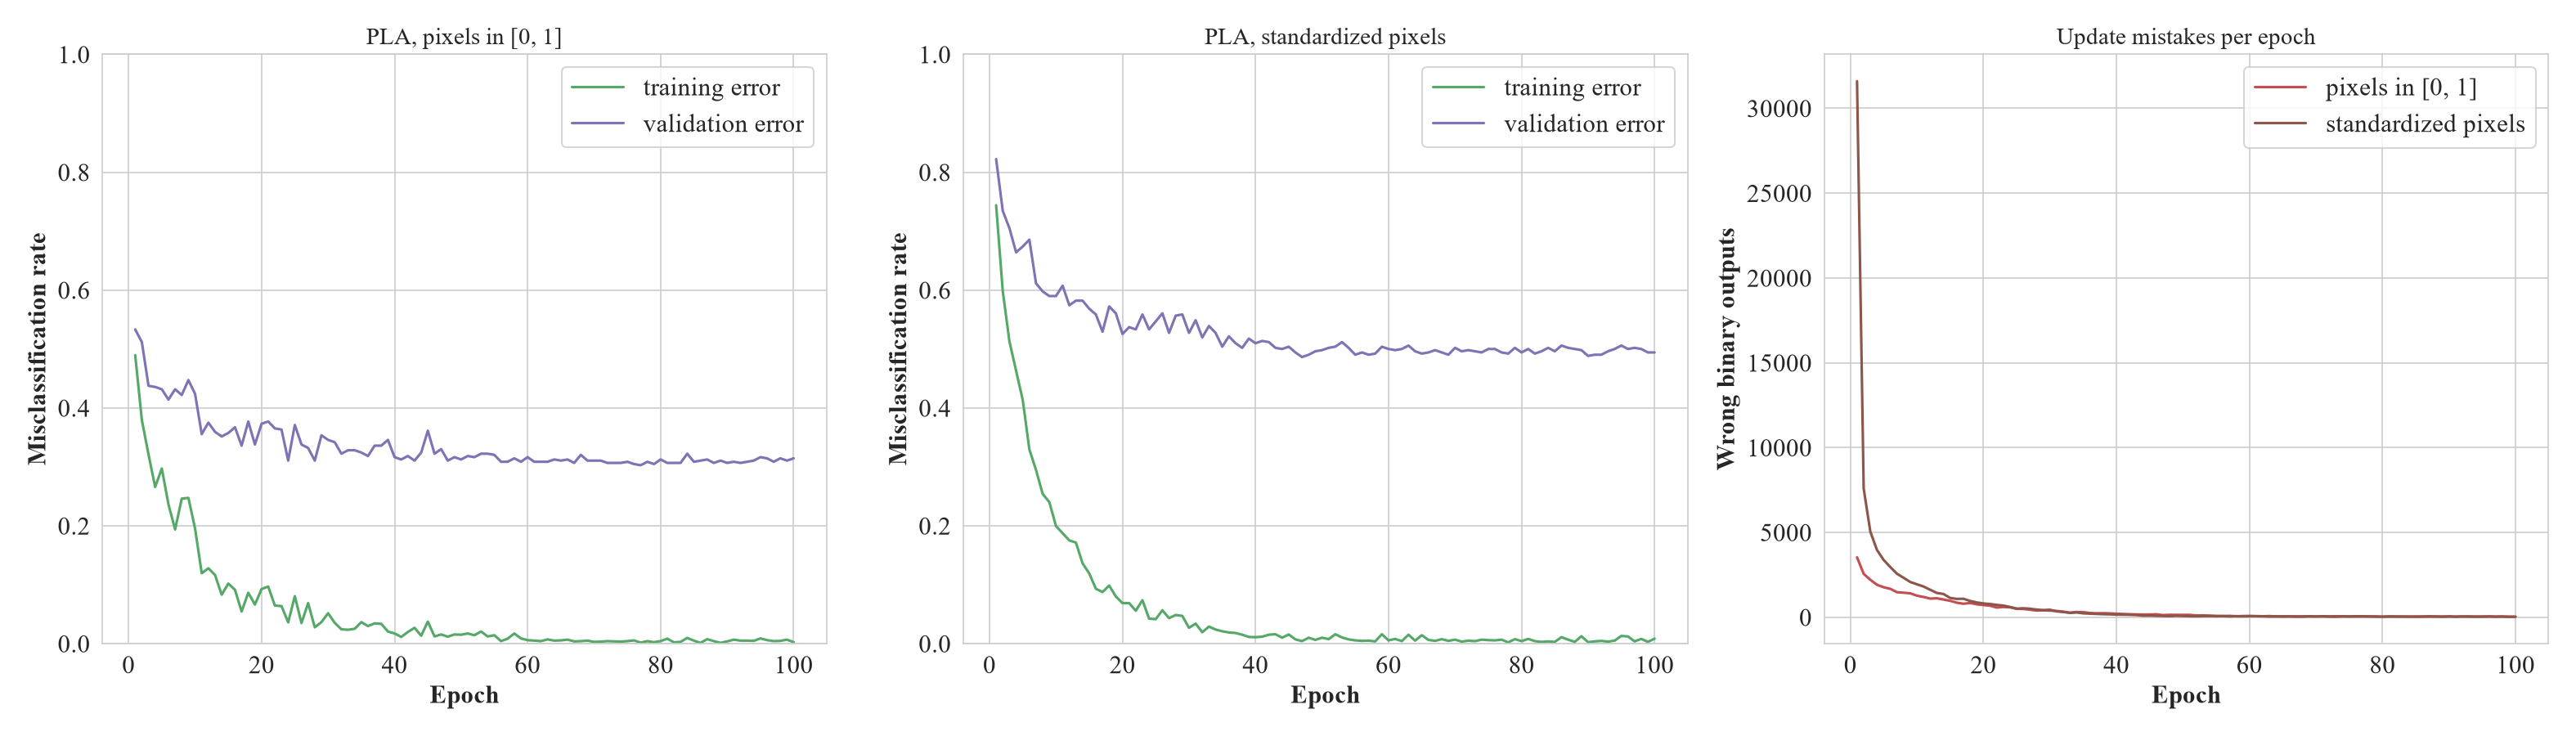
\includegraphics[width=\linewidth]{figures/02_pla_training_curves.png}
\caption{PLA training and validation error against epochs for pixel inputs in $[0,1]$ (left) and
standardized pixels (centre), and the number of wrong binary outputs seen during each epoch's
updates (right).}
\end{figure}
\textbf{Inference:} With $[0,1]$ inputs the training error falls to almost zero by epoch 60 while
the validation error levels off near 0.31, and with standardized inputs it levels off near 0.49, so
the gap between the curves is the perceptron's whole problem. The number of update mistakes drops
sharply in the first ten epochs and then creeps toward zero without reaching it.

\begin{figure}[H]
\centering
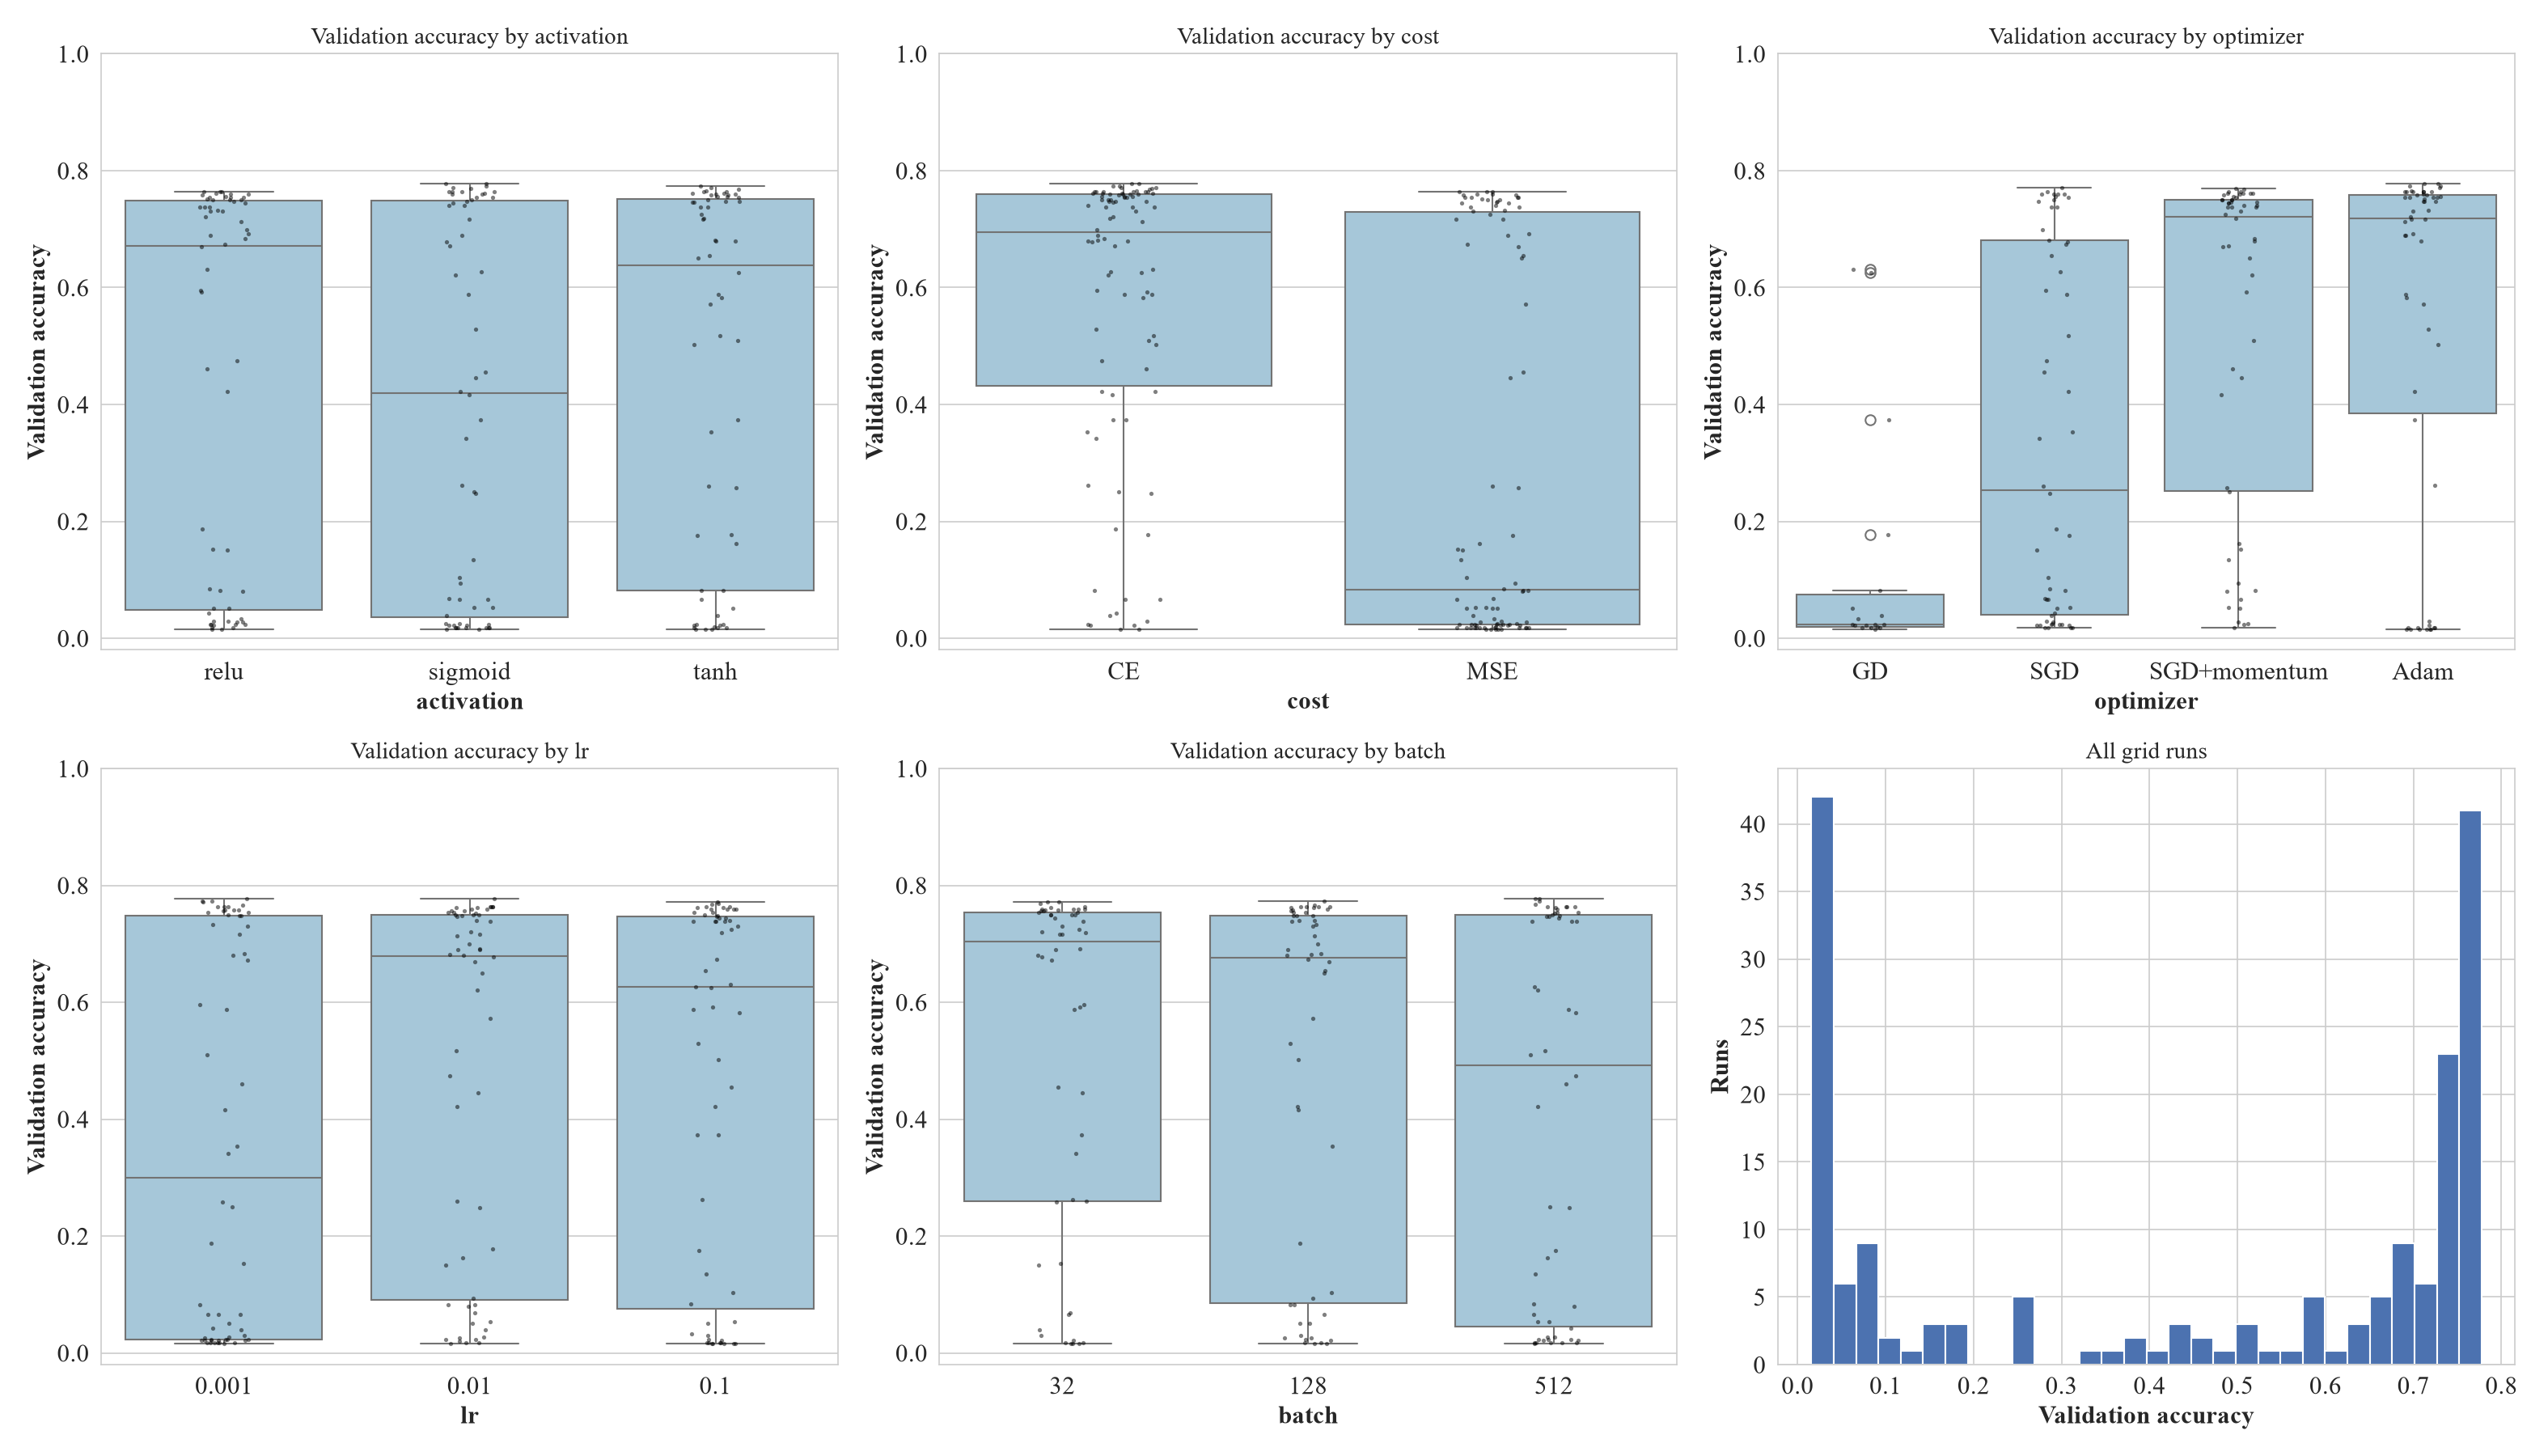
\includegraphics[width=\linewidth]{figures/03_tuning_grid_overview.png}
\caption{Validation accuracy of all 180 grid runs, grouped by each hyperparameter. Dots are
individual runs.}
\end{figure}
\textbf{Inference:} The distribution is bimodal: about 40 runs sit at 2\% to 8\% (failed to train)
and about 40 at 70\% to 78\%, with the rest spread in between. The optimizer panel separates the
groups most clearly. GD is almost entirely in the failed group, plain SGD is spread from failed to
trained (median about 0.25), and momentum SGD and Adam sit mostly near the top (medians about 0.72).
The top edge of every box is about the same for activation, cost, learning rate and batch size, which
agrees with the small best-case spreads in the tables, while the medians and lower edges differ much
more (the MSE median is below 0.1, the CE median near 0.7).

\begin{figure}[H]
\centering
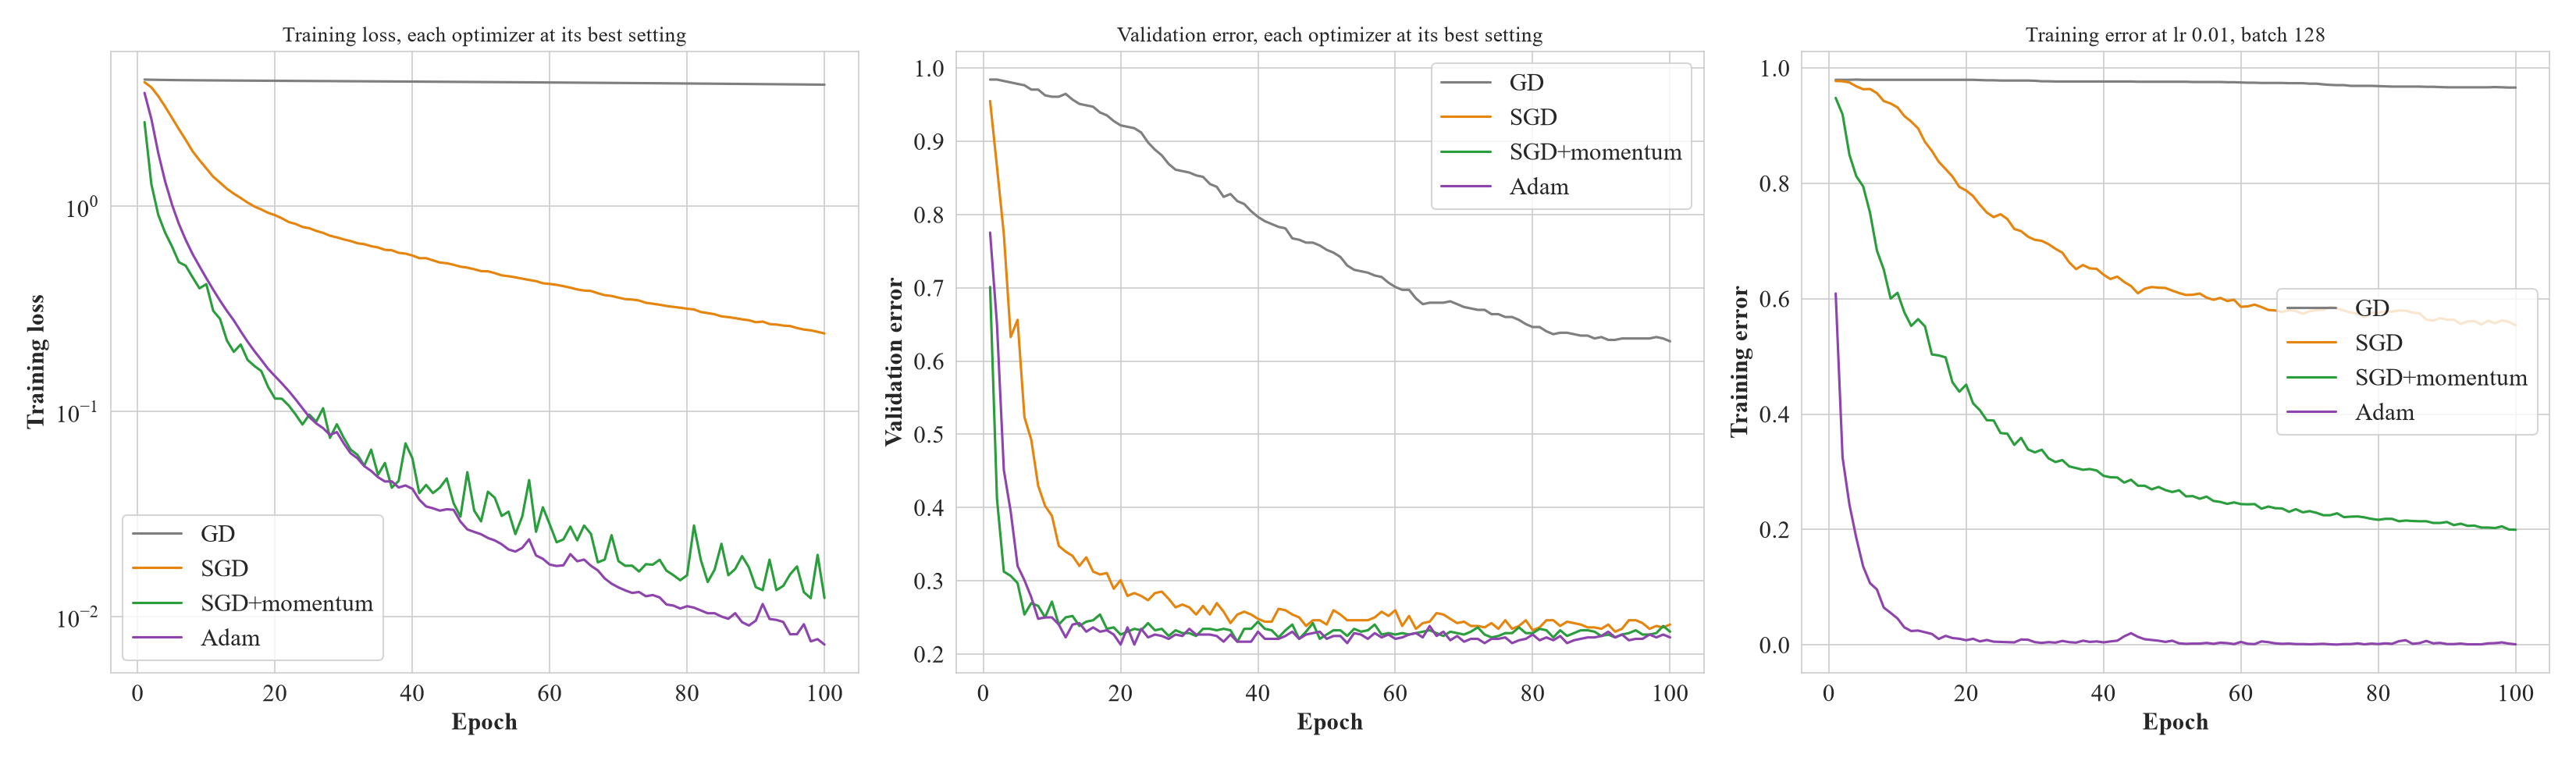
\includegraphics[width=\linewidth]{figures/04_optimizer_convergence.png}
\caption{Left: training loss (log scale) of each optimizer at its own best learning rate and batch
size. Centre: the matching validation error. Right: training error for all four optimizers at the
same learning rate 0.01 and batch 128.}
\end{figure}
\textbf{Inference:} At its own best setting each mini-batch optimizer ends at a similar validation
error (about 0.22 to 0.24), but plain SGD gets there more slowly and its training loss is still far
above Adam's after 100 epochs. Momentum SGD's training loss is noisier from epoch to epoch than
Adam's. At a shared learning rate of 0.01 the difference is stark: Adam's training error is near zero
within about 20 epochs, momentum SGD's is still near 0.20 at epoch 100, plain SGD's is near 0.55, and
GD's is still near 0.97.

\begin{figure}[H]
\centering
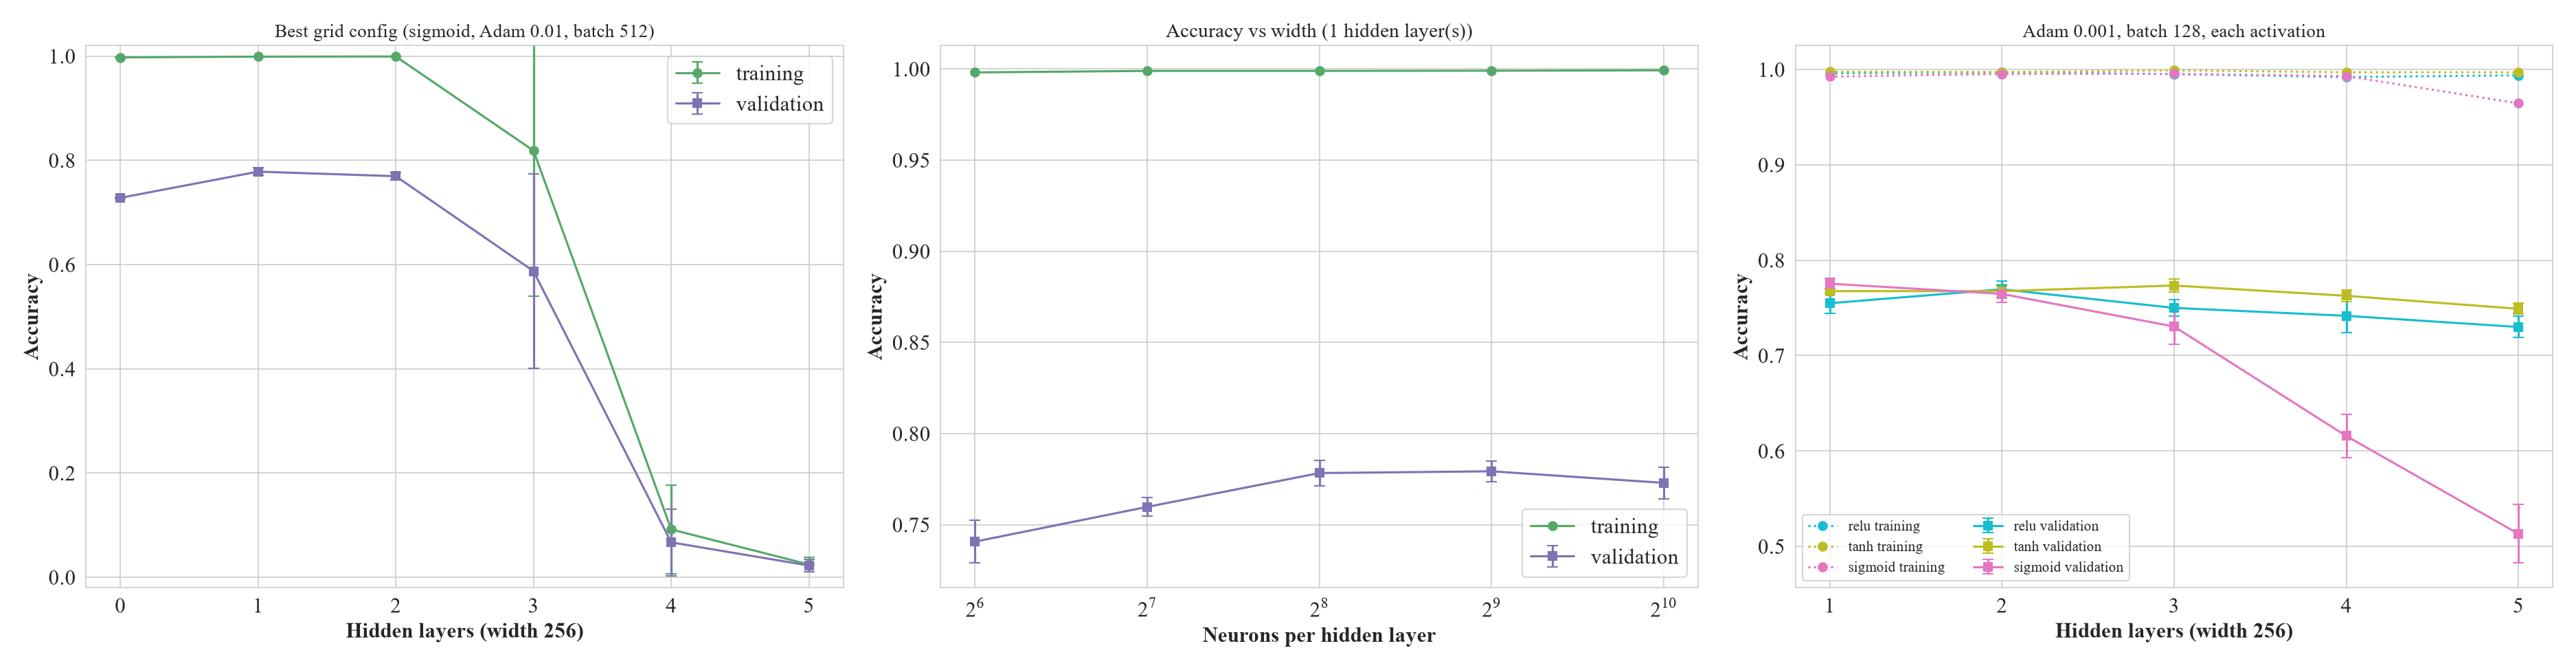
\includegraphics[width=\linewidth]{figures/05_depth_and_width.png}
\caption{Left: accuracy against the number of hidden layers at the grid-winner settings. Centre:
accuracy against width for one hidden layer. Right: accuracy against depth for each activation with
Adam, learning rate 0.001, batch 128. Error bars are one standard deviation over four seeds.}
\end{figure}
\textbf{Inference:} The left panel shows a collapse of both curves from three layers on, the
right panel shows that the collapse is specific to sigmoid at this learning rate: ReLU and tanh
stay near 0.73 to 0.77 at every depth, while sigmoid's validation curve falls steadily.

\begin{figure}[H]
\centering
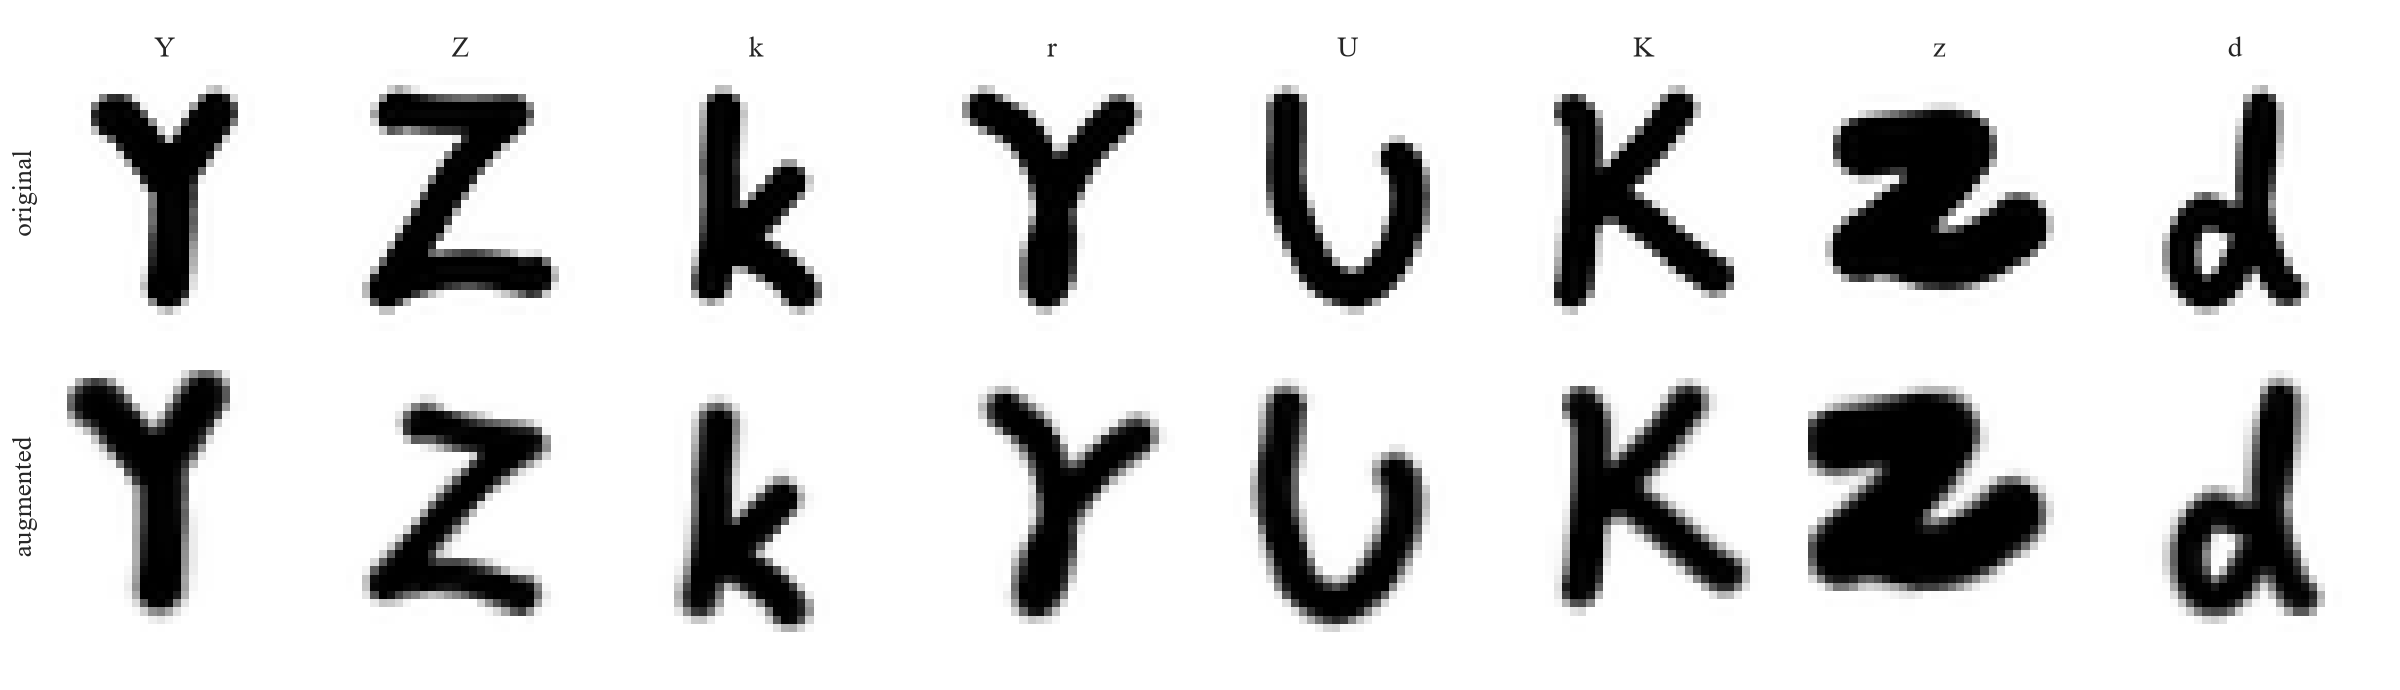
\includegraphics[width=0.85\linewidth]{figures/12_augmentation_examples.png}
\caption{Training images before (top) and after (bottom) the random rotation, scaling and shift
used for augmentation.}
\end{figure}

\begin{figure}[H]
\centering
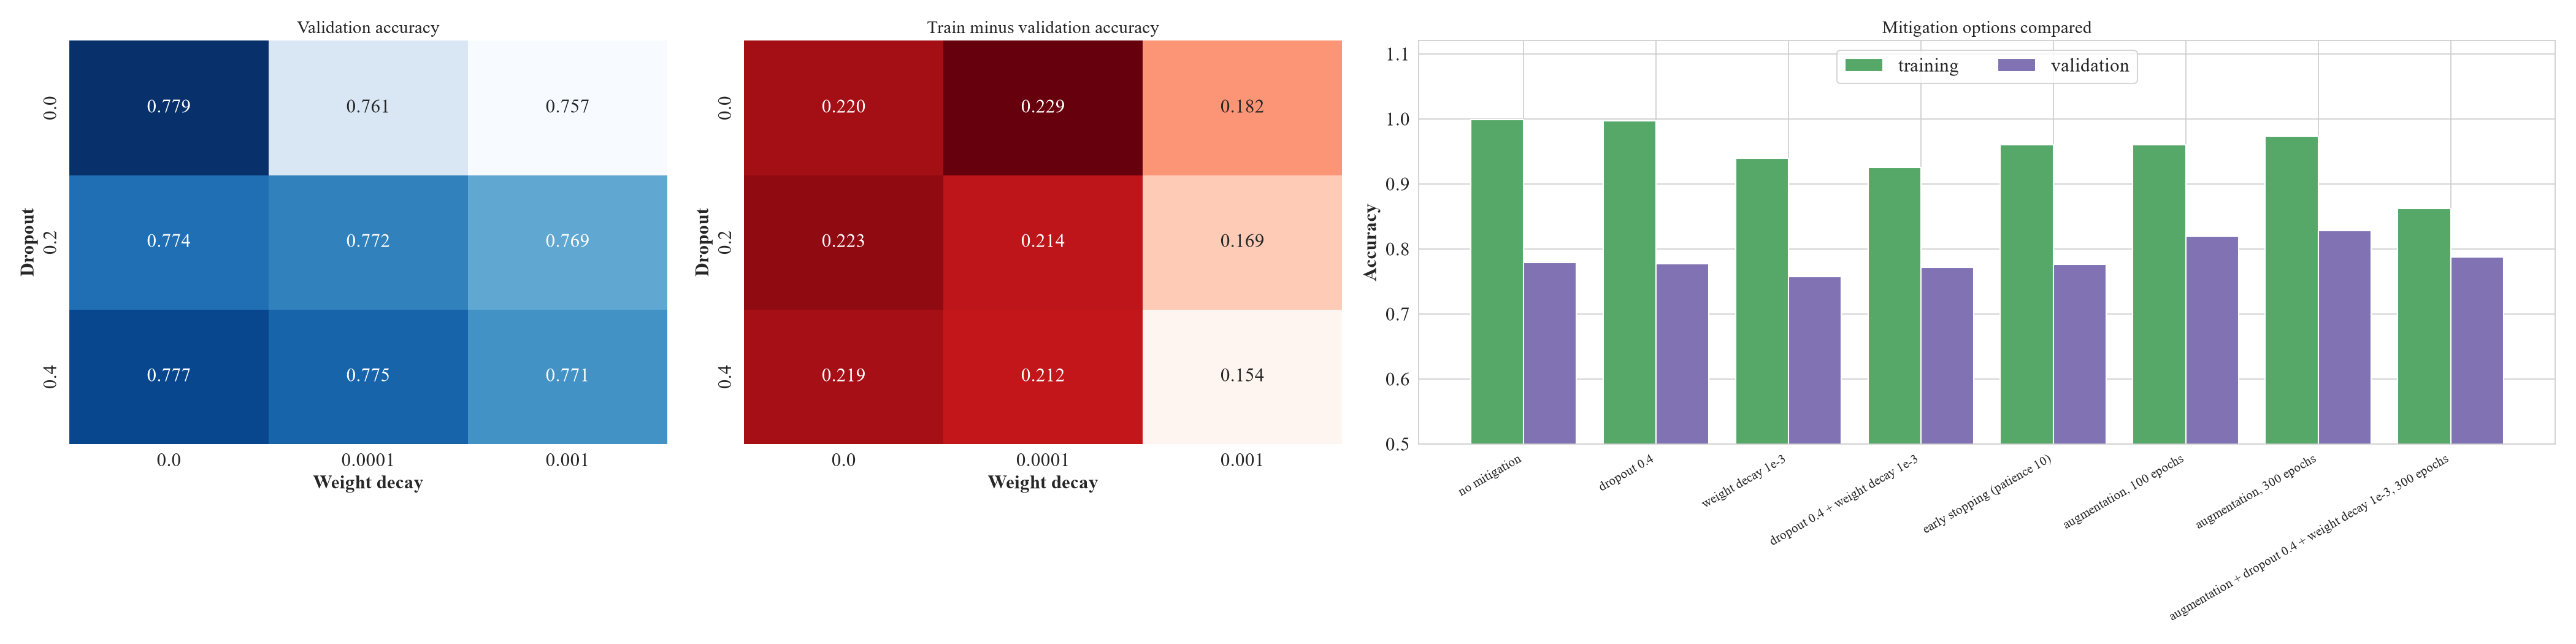
\includegraphics[width=\linewidth]{figures/06_regularization.png}
\caption{Left and centre: validation accuracy and train-minus-validation gap for the dropout and
weight decay grid (100 epochs, no augmentation). Right: training and validation accuracy for every
overfitting remedy tried.}
\end{figure}
\textbf{Inference:} The heatmaps show that the gap shrinks mainly with weight decay and that
validation accuracy is highest with no regularisation at all in that grid. The right panel shows the
one remedy that lifted the validation bars, augmentation, and that the combined
augmentation, dropout and weight decay setting lowered both bars.

\begin{figure}[H]
\centering
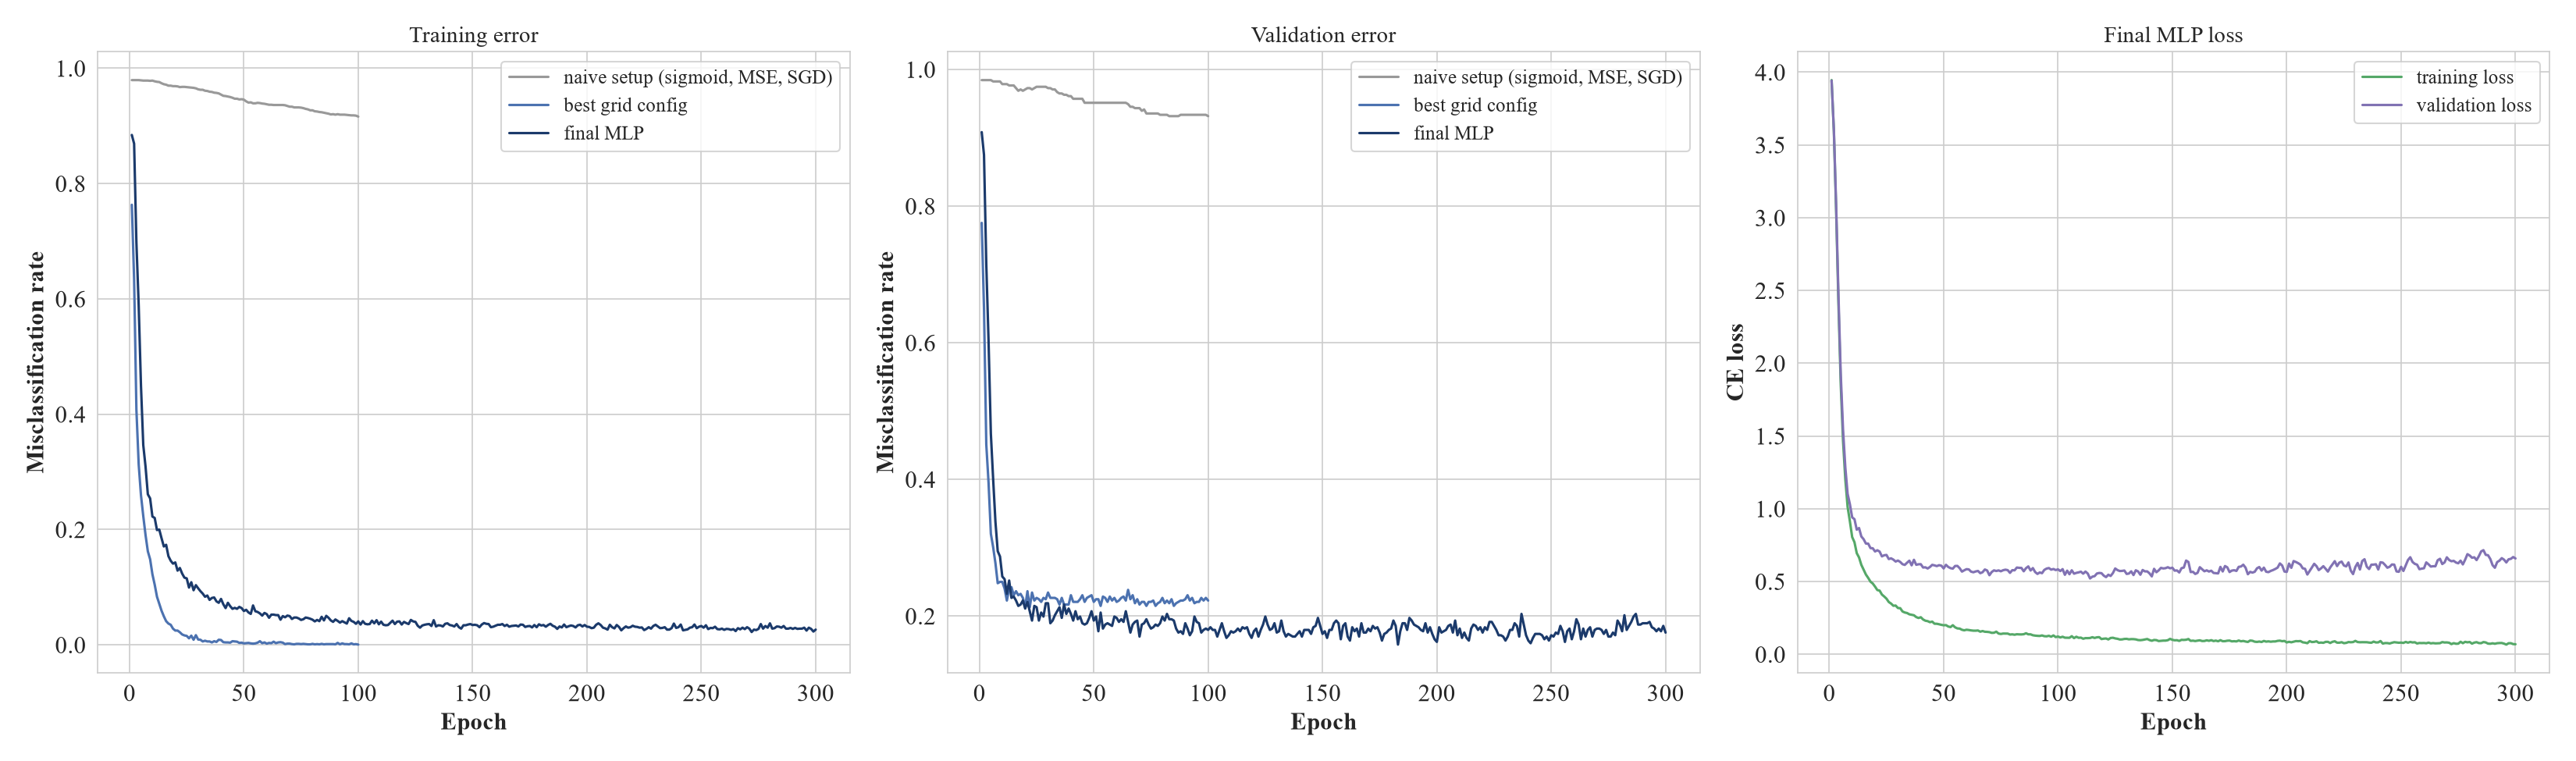
\includegraphics[width=\linewidth]{figures/07_mlp_training_curves.png}
\caption{Training error (left) and validation error (centre) against epochs for the naive setup
(sigmoid, MSE, SGD), the best grid configuration, and the final MLP; and the final MLP's
cross-entropy loss (right).}
\end{figure}
\textbf{Inference:} The naive setup has barely started to learn after 100 epochs, while the best
grid configuration reaches zero training error within about 50 epochs while its validation error
stays near 0.22. The final MLP learns more slowly on the training set, which is expected because
augmented images are harder to fit, but its validation error is lower, around 0.17 to 0.19. In the loss plot the validation
loss stops improving after roughly 100 epochs and drifts upward a little while the training loss
keeps falling, a sign of overfitting that persists even with augmentation.

\begin{figure}[H]
\centering
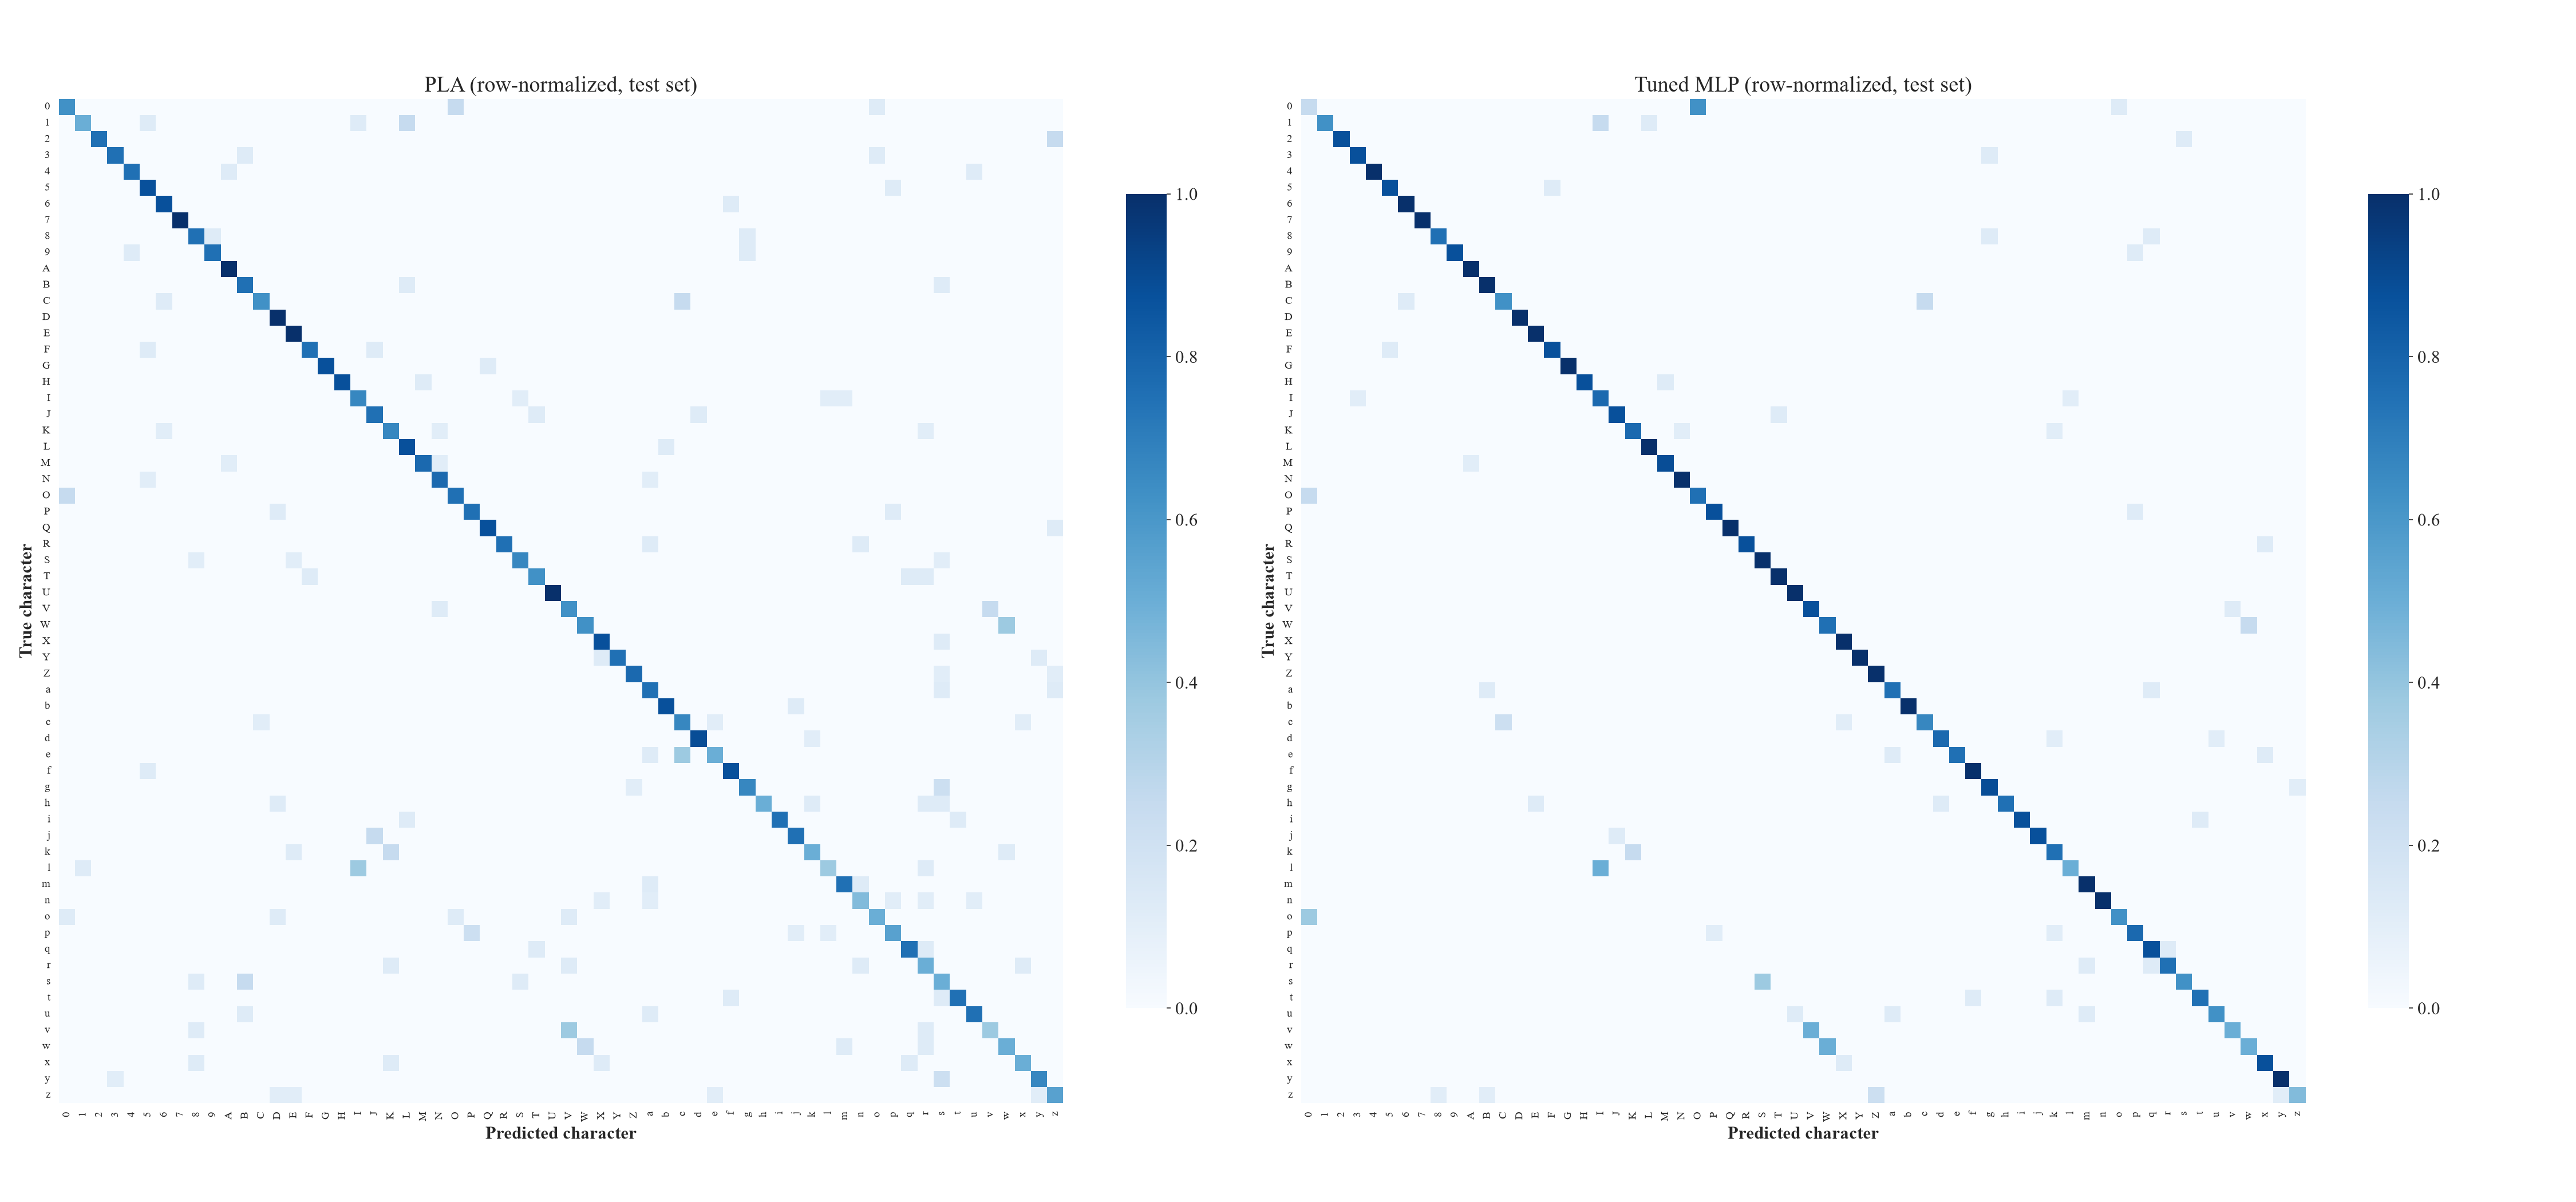
\includegraphics[width=\linewidth]{figures/08_confusion_matrices.png}
\caption{Row-normalised confusion matrices on the test set for the PLA (left) and the tuned MLP
(right). Characters are ordered 0--9, A--Z, a--z.}
\end{figure}
\textbf{Inference:} The MLP's diagonal is darker and its off-diagonal mass is smaller and more
concentrated. Its most visible errors are pairs of look-alike characters: the digit 0 predicted as
the letter O (5 of 8 test images), the letter l as I, o as 0, and the lowercase and uppercase forms of
v, w and s. The perceptron makes the same look-alike mistakes (l as I, W as w, v as V) but adds
confusions between unrelated shapes such as e as c, s as B and y as s, and no single pair
dominates (its most frequent pair occurs 3 times).

\begin{figure}[H]
\centering
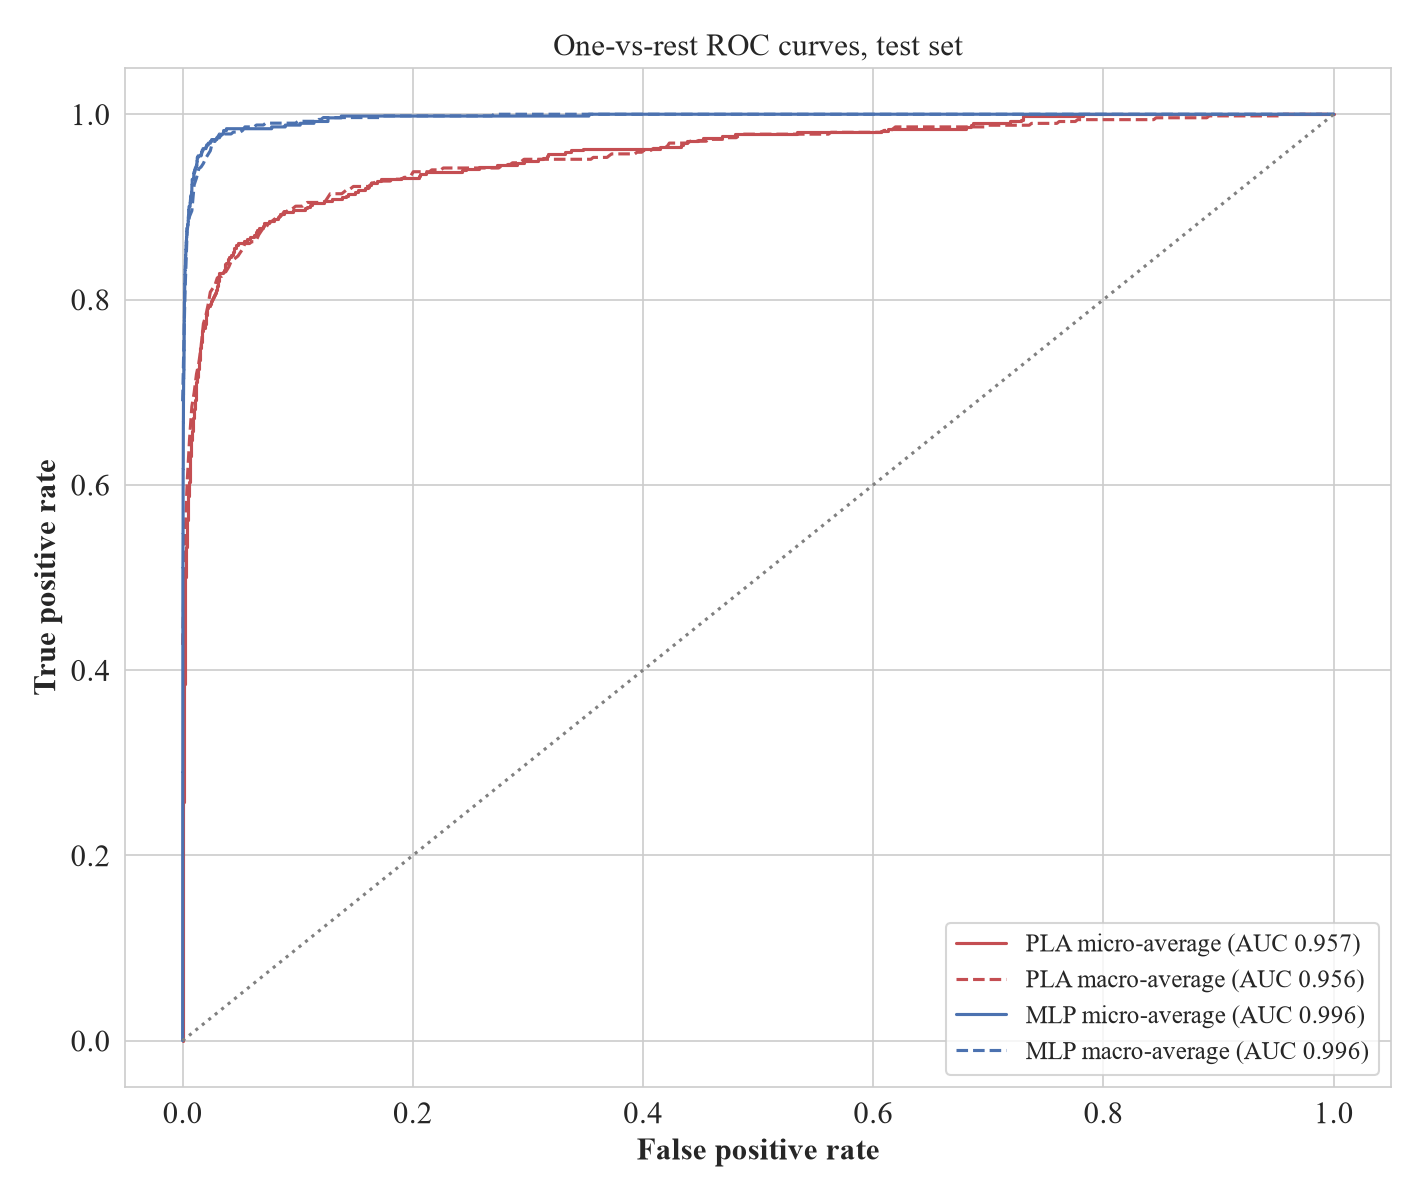
\includegraphics[width=0.75\linewidth]{figures/09_roc_curves.png}
\caption{One-vs-rest ROC curves on the test set, micro-average (solid) and macro-average (dashed),
for the PLA and the MLP.}
\end{figure}
\textbf{Inference:} The micro and macro averages lie almost on top of each other for each model, as
expected with 8 or 9 test images in every class. The MLP curve (AUC 0.9960 micro,
0.9961 macro) rises to a true-positive rate above 0.95 at a false-positive rate
below 0.02, whereas the PLA curve (AUC 0.9565, 0.9558) needs a
false-positive rate near 0.2 to reach 0.93. The perceptron's raw scores from 62 separately trained
heads are not calibrated against each other, which is one reason its ranking quality is lower. The
high AUC values for both models probably also reflect that with 62 classes most negatives are easy
(an inference, not tested).

\begin{figure}[H]
\centering
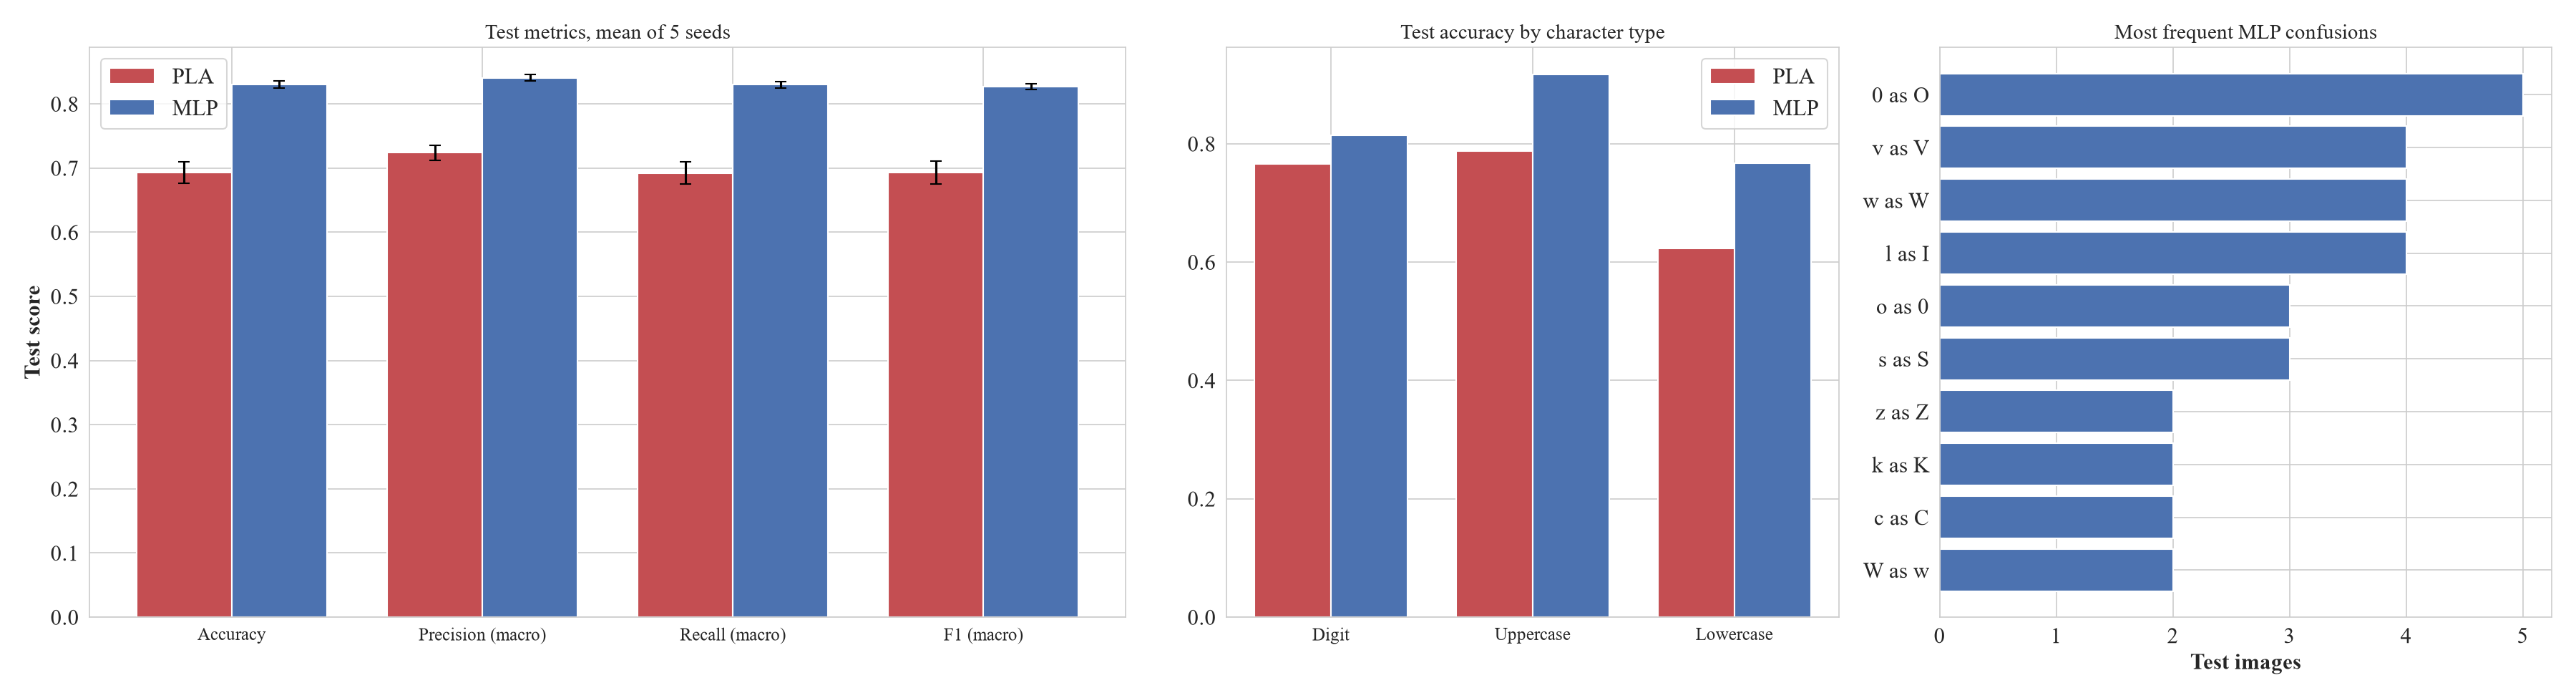
\includegraphics[width=\linewidth]{figures/10_ab_comparison.png}
\caption{Left: test accuracy, macro precision, macro recall and macro F1 for the PLA and the MLP
(mean of five seeds, error bars one standard deviation). Centre: test accuracy by character type.
Right: the ten most frequent MLP confusions.}
\end{figure}

\begin{figure}[H]
\centering
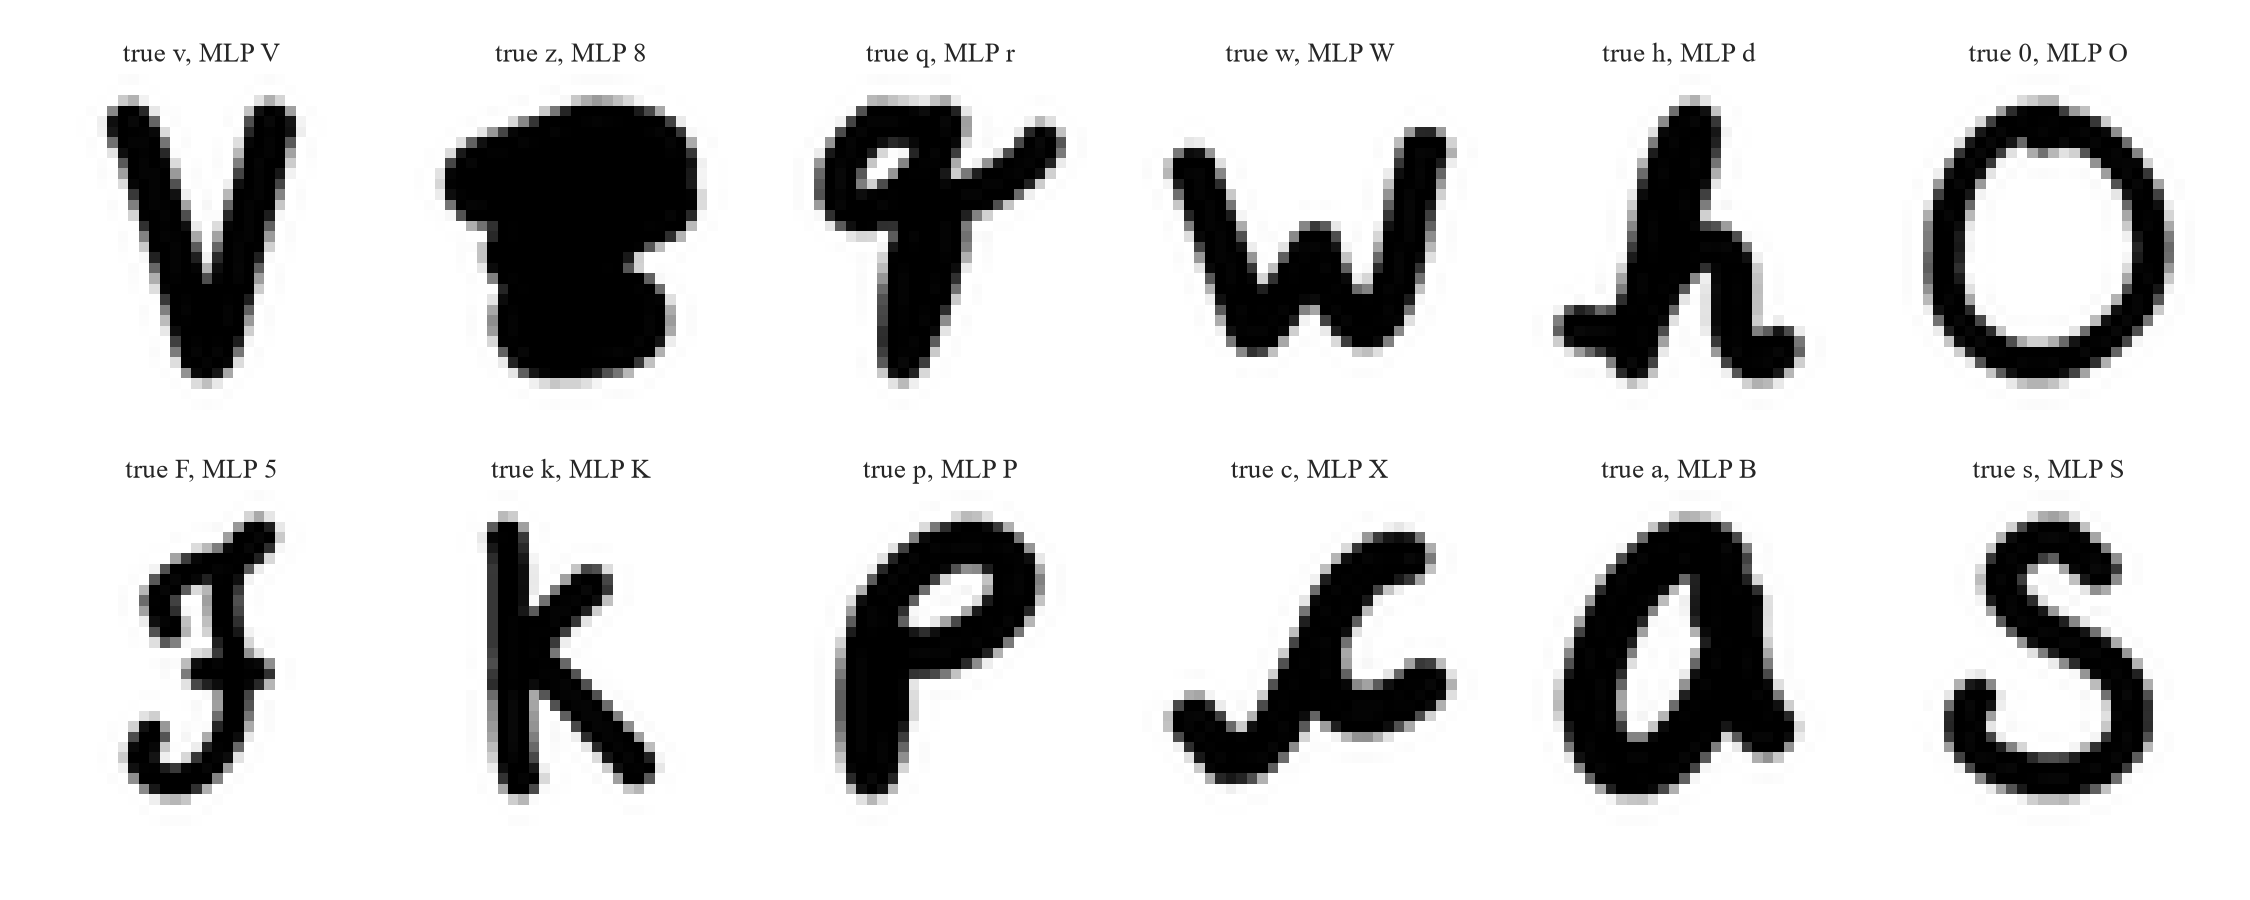
\includegraphics[width=0.9\linewidth]{figures/11_mlp_errors.png}
\caption{Twelve of the MLP's misclassified test images (seed 42), with the true and predicted
character.}
\end{figure}
\textbf{Inference:} Several of these are cases where the character cannot be identified without
its size, since the pipeline scales every character to fill the same $32 \times 32$ square (v and V,
w and W, s and S, k and K, p and P). This is an explanation inferred from the images and from the
class-mean correlations in the EDA section; it was not tested by keeping size as a feature. Others
are hard to read even for a person (the filled blob labelled z, the cursive F read as a 5, and the c
that looks like an x).

\section{Discussion}

\subsection*{Strengths and weaknesses of PLA and MLP}
\begin{longtable}{p{2.3cm}p{5.9cm}p{6.2cm}}
\toprule
 & PLA & MLP \\
\midrule
Strengths & A short \texttt{numpy} class, no gradients. Learning rate is irrelevant with zero
initialisation. 3.7 s for 77 epochs on the CPU. & 83.0\%
test accuracy, ROC AUC 0.9960, more stable across seeds. Smooth loss allows
optimizers, regularisation and augmentation. \\
Weaknesses & 69.3\% test accuracy, larger seed-to-seed variation, raw
scores that are not calibrated, no convergence guarantee on this data, and worse with standardized
inputs. & Many interacting hyperparameters (the naive setup reached 6.8\%); overfits
(train-validation gap of 14.6 points even after mitigation);
556,606 weights against 63,550. \\
\bottomrule
\end{longtable}
The timing rows are not a like-for-like comparison: the perceptron ran on the CPU and the MLP on the
GPU (2.2 s for 300 epochs).

\subsection*{Observation Questions}
\textbf{1. Why does PLA underperform compared to MLP?} Not because it cannot fit the data: its
training accuracy is 99.2\%. It generalises worse
(69.3\% test accuracy against 83.0\%) for
several measured reasons. First, it is a single linear layer on raw pixels, and a plain softmax
classifier with the same weights already scores 72.0\%, so the
representation limit is a large part of the ceiling. Second, the perceptron only updates on mistakes
and has no loss to minimise, so the boundary stops improving once the training images are
nearly separated and it ends up wherever the last mistake left it. That is consistent with its larger
variation across shuffle orders (1.7 points against
0.5) and with the extra 2.7
points the softmax classifier gains on the test set. Third, a hidden layer lets the MLP build
intermediate features from strokes: on the test set the hidden layer added
5.9 points over the softmax
classifier (5.0 on validation). Fourth, the MLP was also trained
with data augmentation, worth a further 5.2
points on the test set; this was not tried with the perceptron. The four measurements are the
accuracies above; that the hidden layer's benefit comes from stroke-like features is an inference.

\textbf{2. Which hyperparameters had the most impact on MLP performance?} The optimizer and its
learning rate, and the cost function. Over the grid the optimizer had the largest spread in mean
validation accuracy (0.421), followed by the cost function
(0.261); moving away from the best configuration, switching to GD,
plain SGD or momentum SGD cost 15.6 to
73.8 points, a learning rate of 0.1 cost
18.9, and batch size 32 cost 8.8 points. The
activation function mattered least (at most 2.3 points at the
best setting). Among the design choices outside the grid, the presence of a hidden layer
(5.0 points), the width (3.9 points
from 64 to 512 neurons) and data augmentation
(4.8 points) each moved
validation accuracy by more than the choice of activation or cost did once training worked at all.
The caveat is that the mean spreads are inflated by runs that failed to train, and single-seed
differences under about one point are within noise.

\textbf{3. Did optimizer choice (SGD vs Adam) affect convergence?} Yes, strongly for speed and
reliability, little for final accuracy. At learning rate 0.01 and batch 128, Adam reached
99.9\% training accuracy in 100 epochs while plain SGD reached
44.6\%. Plain SGD needed a learning rate of 0.1 and batch size 32 to do
well, and even then took 64 epochs to reach 90\% training
accuracy, against 12 for Adam (both at the setting with the best
validation accuracy).
Only 1 of the 9 plain-SGD settings reached that level, compared with
6 of 9 for Adam. Given each one's best learning rate, the final
validation accuracies were close (76.0\% for SGD,
77.0\% for momentum, 77.7\% for Adam).
Momentum SGD converged nearly as fast as Adam (11
epochs to 90\% training accuracy), which suggests that most of Adam's advantage over plain SGD in
this experiment is momentum-like smoothing plus insensitivity to the learning rate.

\textbf{4. Did adding more hidden layers always improve results?} No. With the grid-winner
settings the second hidden layer did not improve validation accuracy
(77.8\% to 77.0\%, within the seed noise), three layers trained in
some seeds and not in others (training accuracy 81.9\% with a standard deviation of
28.0 points), and four or more layers failed to train at all. With the gentler Adam 0.001 settings, every network trained, and for ReLU and tanh the validation
accuracy differed by at most 4.0 points between any two depths: ReLU improved from
one to two layers and then declined, and tanh was flat within noise up to three layers and declined
afterwards. Sigmoid declined steadily, by 26.2
points from one to five layers. The train-validation gap widened with depth for ReLU
(24.1 to 26.4 points) and sigmoid
(21.7 to 45.1). Plausible reasons are that the
training set is small (2386 images, about 38 per class) so extra capacity is not backed by extra
information, and that deeper networks are harder to optimise; only the second was directly
observed (the failed sigmoid runs), the first is an interpretation.

\textbf{5. Did the MLP show overfitting? How could it be mitigated?} Yes. The best configuration
reaches 99.9\% training accuracy against
77.9\% validation accuracy. Of the remedies tried, only data
augmentation improved validation accuracy (to 82.8\%, and on
the test set the final model scored 83.0\%). Dropout and early stopping
did not help on their own, weight decay reduced the gap but lowered accuracy, and stacking every
remedy together underfitted. Overfitting was reduced, not removed: the final model still has a
train-validation gap of 14.6 points and its validation loss
rises slowly late in training. More training data, or stronger and better-matched augmentation, are
the obvious next steps, but were not tried.

\subsection*{Limitations}
The test set has 512 images (one image is 0.2 points), only one train, validation and test split was
used, and each model was run with five seeds, so differences below about two points between the
softmax classifier and the perceptron should not be over-read. Augmentation and the overfitting study
were carried out only for the MLP, so the perceptron was not given the same chances to improve. The
grid used a single seed per run and a single width (256), so the ranking of near-equal configurations
is not reliable. The preprocessing removes the size of a character, which may cost accuracy on case
pairs.

\section{Conclusion}
A perceptron written from scratch reached 69.3\% test accuracy
(macro F1 0.6931) on 62-class handwritten character recognition, while a tuned
MLP reached 83.0\% (macro F1 0.8273); the ROC AUC
rose from 0.9565 to 0.9960. The perceptron fits the training images
almost perfectly and generalises badly. A linear softmax classifier with the same number of weights
closes only part of the gap (72.0\%); the hidden layer adds
5.9 more points
(77.9\%) and augmentation, which was tried only with the MLP, a
further 5.2. Tuning was decisive for the MLP: an untuned textbook setup (sigmoid, MSE,
SGD) reached 6.8\% validation accuracy, whereas Adam with cross-entropy reached
about 77.8\%. The optimizer and its learning rate had the largest effect;
the activation function had little. More hidden layers did not help, and the MLP overfits, with
data augmentation the only remedy that improved validation accuracy. The chosen model is one hidden
layer of 512 sigmoid units, cross-entropy, Adam with learning rate 0.01, batch size 512, and
augmentation for 300 epochs. About a third of its remaining test errors (28 of 83) are a letter
predicted as its other-case twin, and the most frequent single confusion is the digit 0 predicted as
the letter O.




\section{References}
\begin{enumerate}
\item Dhruvil Dave, ``English Handwritten Characters Dataset,'' Kaggle. [Online]. Available:
\url{https://www.kaggle.com/datasets/dhruvildave/english-handwritten-characters-dataset}
\item F. Rosenblatt, ``The Perceptron: A Probabilistic Model for Information Storage and
Organization in the Brain,'' \emph{Psychological Review}, vol. 65, no. 6, pp. 386--408, 1958.
\item D. E. Rumelhart, G. E. Hinton, and R. J. Williams, ``Learning representations by
back-propagating errors,'' \emph{Nature}, vol. 323, pp. 533--536, 1986.
\item D. P. Kingma and J. Ba, ``Adam: A Method for Stochastic Optimization,'' in \emph{Proc. 3rd
International Conference on Learning Representations (ICLR)}, 2015.
\item N. Srivastava, G. Hinton, A. Krizhevsky, I. Sutskever, and R. Salakhutdinov, ``Dropout: A
Simple Way to Prevent Neural Networks from Overfitting,'' \emph{Journal of Machine Learning
Research}, vol. 15, pp. 1929--1958, 2014.
\item A. Paszke et al., ``PyTorch: An Imperative Style, High-Performance Deep Learning Library,''
in \emph{Advances in Neural Information Processing Systems 32}, 2019.
\item Scikit-learn Developers, ``Metrics and scoring,'' Scikit-learn Documentation. [Online].
Available: \url{https://scikit-learn.org/stable/modules/model_evaluation.html}
\end{enumerate}

\end{document}
